\documentclass{libs/XJTLU_format}
% Inserting the preamble file with the packages
%%%%%%%%%%%%%%%%%%%%%%%%%%%%%%%%%%%%%%%%%%%%%%%%%%%%%%%%%%%%%%%%%%%%%
%% This file contains the packages that can be used in the beamer. %%
%%%%%%%%%%%%%%%%%%%%%%%%%%%%%%%%%%%%%%%%%%%%%%%%%%%%%%%%%%%%%%%%%%%%%
\usepackage[english,brazil]{babel}
% Package to fonts family
\usepackage[T1]{fontenc}
% Package to accentuation
\usepackage[utf8]{inputenc}
% Package to Figures
\usepackage{graphicx}
\graphicspath{{./images/}}
% Package to the colors
\usepackage{color}
% Package to the colors
\usepackage{xcolor}
% Packages to math symbols and expressions
\usepackage{amsfonts, amssymb, amsmath}
% Package to multiple lines and columns in table
\usepackage{multirow, array} 
% Package to create pseudo-code
% For more detail of this package: http://linorg.usp.br/CTAN/macros/latex/contrib/algorithm2e/doc/algorithm2e.pdf
\usepackage{algorithm2e}
% Package to insert code
\usepackage{listings} 
\usepackage{keyval}
% Package to justify text
\usepackage[document]{ragged2e}
% Package to manage the bibliography
\usepackage[backend=biber, style=numeric, sorting=none]{biblatex}
% Package to facilities quotations
\usepackage{csquotes}
% Package to use multicols
\usepackage{multicol}
\usepackage{transparent}

% Inserting the references file
\bibliography{libs/references.bib} 

% Title
\title[Defesa de Projeto de Graduação]{\normalsize\textbf{Desenvolvimento de Base de Dados para Treinamento de Redes Neurais de Reconhecimento de Voz
Através da Geração de Áudios com Resposta ao Impulso Simuladas por Técnicas de Data Augmentation}}
% Subtitle
%\subtitle{Creating Presentations}
% Author of the presentation
\author{Bruno Machado Afonso} 

% Institute's Name
\institute[- Escola Politécnica]{
    % email for contact
    \email{bruno.ma@poli.ufrj.br}
    \newline
    % Department Name
    \department{\scriptsize Departamento de Engenharia Eletrônica e de Computação - Escola Politécnica}
    \newline
    % University name
    \university{\scriptsize Universidade Federal do Rio de Janeiro}
}
% date of the presentation
\date{\today}


%%%%%%%%%%%%%%%%%%%%%%%%%%%%%%%%%%%%%%%%%%%%%%%%%%%%%%%%%%%%%%%%%%%%%%%%%%%%%%%%%%
%% Start Document of the Presentation                                           %%               
%%%%%%%%%%%%%%%%%%%%%%%%%%%%%%%%%%%%%%%%%%%%%%%%%%%%%%%%%%%%%%%%%%%%%%%%%%%%%%%%%%
\begin{document}
%%%%%%%%%%%%%%%%%%%%%%%%%%%%%%%%%%%%%%%%%%%%%%%%%%%%%%%%%%%%%%%%%%%%%%%%%%%%%%%%%%%
%% This file contains the style of the codes show in slides.                     %%
%% The package used is listings, but it possible to used others.                 %%
%%%%%%%%%%%%%%%%%%%%%%%%%%%%%%%%%%%%%%%%%%%%%%%%%%%%%%%%%%%%%%%%%%%%%%%%%%%%%%%%%%%

% color used in the code style
\definecolor{codegreen}{rgb}{0,0.6,0}
\definecolor{codegray}{rgb}{0.5,0.5,0.5}
\definecolor{codepurple}{rgb}{0.58,0,0.82}
\definecolor{codebackground}{rgb}{0.95,0.95,0.92}

% style of the code!
\lstdefinestyle{codestyle}{
    backgroundcolor=\color{codebackground},   
    commentstyle=\color{codegreen},
    keywordstyle=\color{magenta},
    numberstyle=\tiny\color{codegray},
    stringstyle=\color{codepurple},
    basicstyle=\ttfamily\footnotesize,
    frame=single,
    breakatwhitespace=false,         
    breaklines=true,                 
    captionpos=b,                    
    keepspaces=true,                 
    numbers=left,                    
    numbersep=5pt,                  
    showspaces=false,                
    showstringspaces=false,
    showtabs=false,                  
    tabsize=2,
    title=\lstname 
}

\lstset{style=codestyle}


%% ---------------------------------------------------------------------------
% Título
\begin{frame}{}
    
\includegraphics[scale=0.1]{minerva-ufrj.png} \hspace{3cm} \vspace{-0.2cm}
    
\includegraphics[scale=0.15]{poli.png} \hspace{2cm} \vspace{-0.2cm}
    
\includegraphics[scale=0.25]{del.png} \hspace{-0.1cm} \vspace{-0.1cm}
    \maketitle
\end{frame} 

%% ---------------------------------------------------------------------------
% Sumário
\begin{frame}{Sumário}
    %\begin{multicols}{2}
        \tableofcontents
    %\end{multicols}
\end{frame}

%% ---------------------------------------------------------------------------
% SECTION: Motivação
\section{Motivação}

\begin{frame}{Motivação}
    Crescimento no número de aplicações de algoritmos de processamento de áudio.
    \vspace{0.5cm}

    \begin{itemize}
        \item Detecção e reconhecimento de voz\begin{itemize}
            \item Smartphones
            \item Automação residencial
            \item Comunicação online
        \end{itemize}
        \item Cancelamento de eco 
        \item Separação de fontes
    \end{itemize}
\end{frame}

\begin{frame}{Deep Learning}
    Aumento no número de artigos que envolvem \textit{deep learning} publicados em grandes conferências.
    \vspace{0.5cm}

    \begin{figure} 
        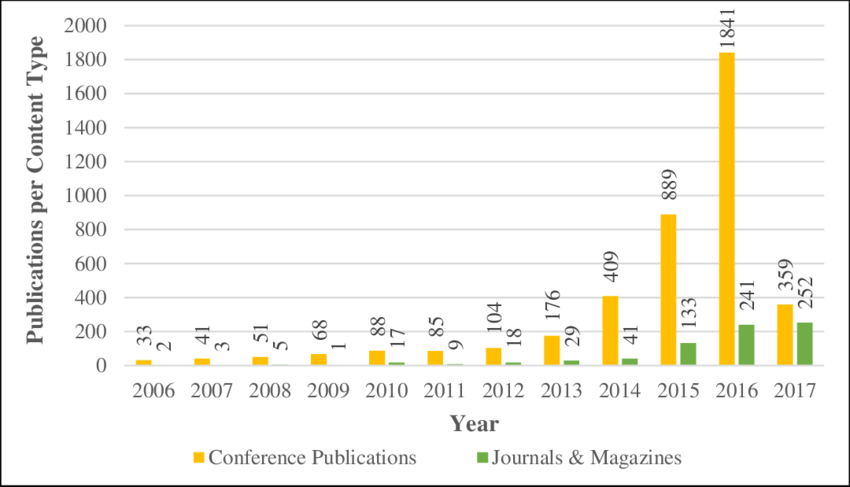
\includegraphics[scale=0.25]{pub_DL_IEEE.png}
        \label{fig:pub_DL_IEEE}
    \end{figure}
\end{frame}

\begin{frame}{Amostra de Voz em Campo Distante (AVCD)}
    Sinal de voz anecóico que é corrompido pela reverberação do ambiente fechado e ruído.
    \vspace{0.5cm}

    \begin{figure}
        \begin{subfigure}{.4\textwidth}
            \centering
            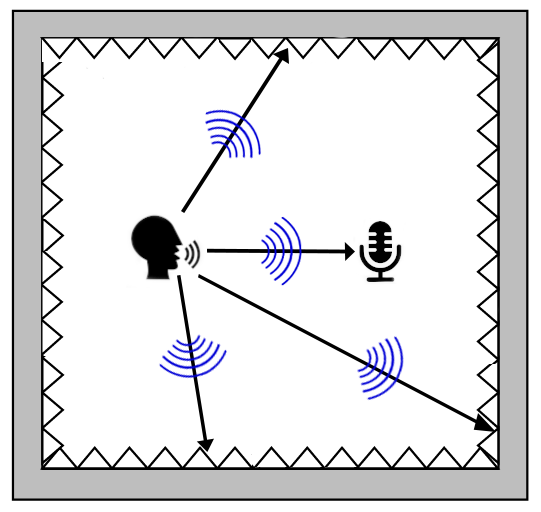
\includegraphics[scale=0.2]{camara_anecoica.png}
            \caption{Sala anecóica}    
        \end{subfigure}
        \begin{subfigure}{.4\textwidth}
            \centering
            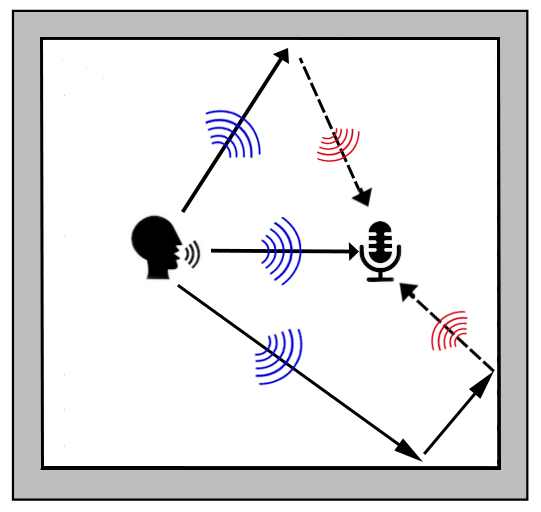
\includegraphics[scale=0.2]{camara_reverb.png}
            \caption{Sala reverberante}    
        \end{subfigure}
        \label{fig:Rooms}
    \end{figure}
\end{frame}

\begin{frame}{Amostra de Voz em Campo Distante (AVCD)}
    \begin{equation*} \label{eqn:model}
        Y(t) = s(t) \ast h(t) + n(t)
    \end{equation*}
    \vspace{0.5cm}

    $Y(t) \rightarrow$  AVCD \\
    $s(t) \rightarrow$  Amostra de Voz Anecóica \\
    $h(t) \rightarrow$  Resposta ao Impulso de Sala (RIR) \\
    $n(t) \rightarrow$  Sinal de Ruído \\
    
\end{frame}

\begin{frame}{Resposta ao Impulso de Sala (RIR)}
    Representa um modelo acústico de um ambiente para um par fonte/receptor.
    \vspace{0.1cm}

    \begin{itemize}
        \item Razão Direto-Reverberante (DRR)
        \item Tempo de Reverberação (T60)
    \end{itemize}

    \begin{figure} 
        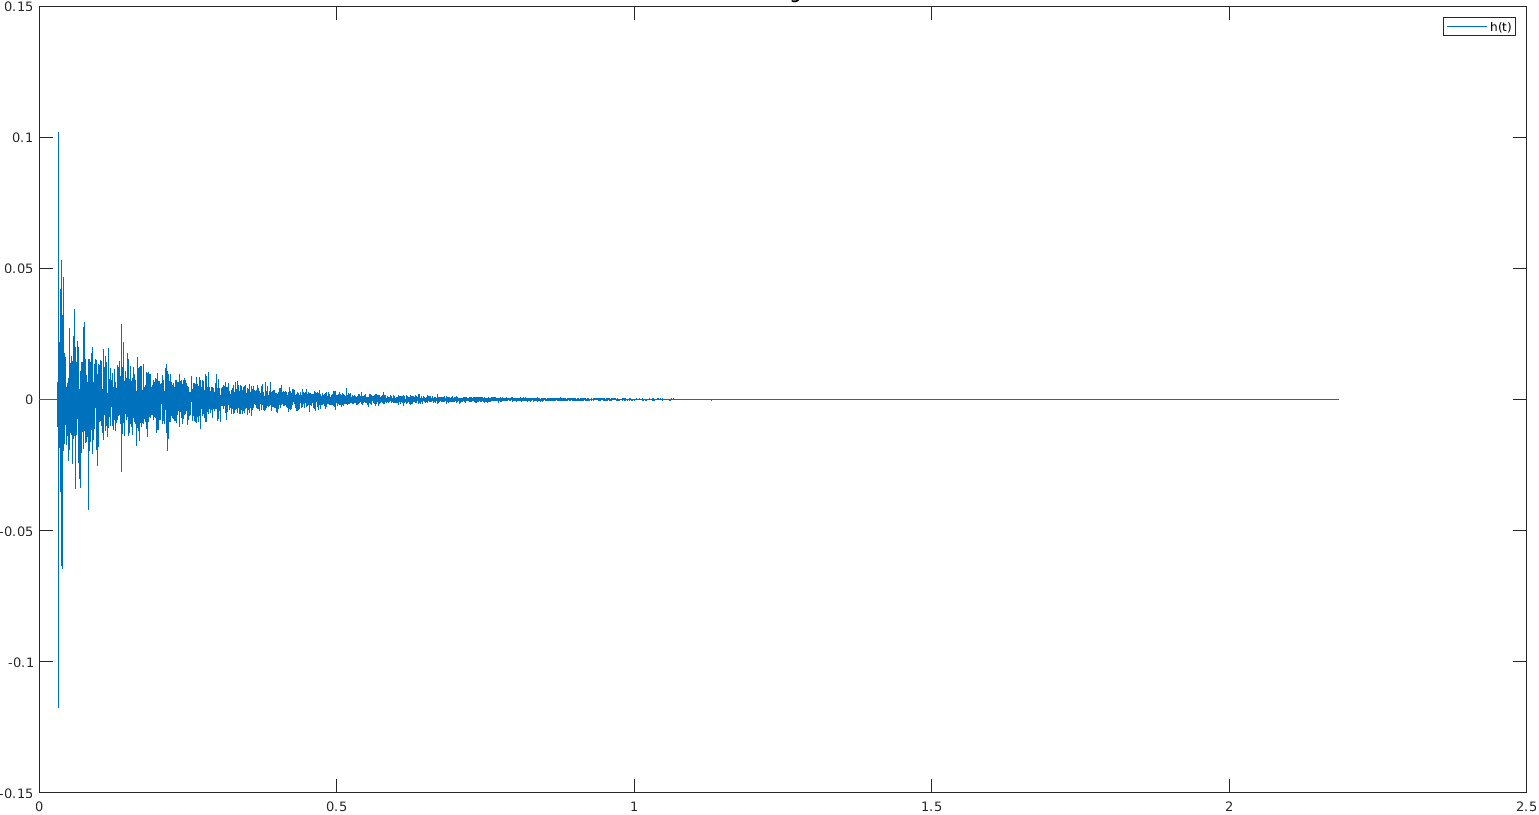
\includegraphics[scale=0.14]{rir-example.png}
        \caption{$DRR = -4,5$ dB / $T60 = 1,38$ s}
        \label{fig:rir-example}
    \end{figure}
\end{frame}

\begin{frame}{Desafios}
    \begin{itemize}
        \item Baixa quantidade e variedade de bases de dados contendo RIRs anotadas para treinamento de redes de \textit{deep learning}.
        \item Dificuldade para realizar gravações de RIRs (equipamentos especializados, variedade de ambientes, etc.)
    \end{itemize}
    \vspace{0.5cm}

    \begin{figure}
        \begin{subfigure}{.45\textwidth}
            \centering
            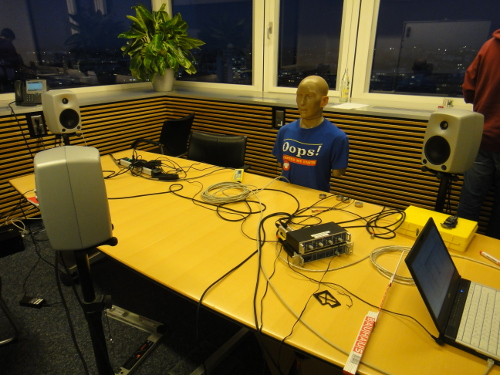
\includegraphics[scale=0.25]{recording.jpg}
        \end{subfigure}
        \begin{subfigure}{.45\textwidth}
            \centering
            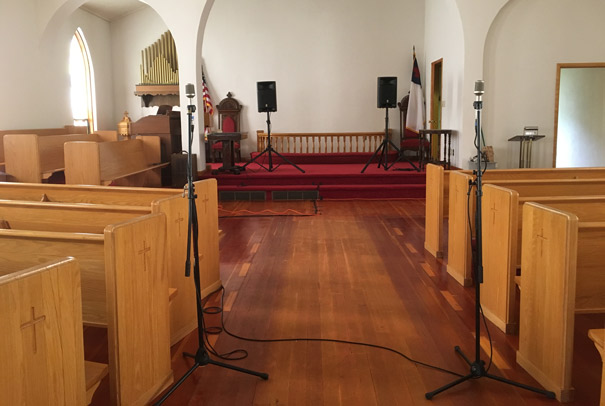
\includegraphics[scale=0.25]{recording3.jpg}
        \end{subfigure}
        \label{fig:recording}
    \end{figure}
\end{frame}

%% ---------------------------------------------------------------------------
% SECTION: Metodologia
\section{Metodologia}

% \begin{frame}{Motivação}
%     Crescimento no número de aplicações de algoritmos de processamento de áudio.
%     \vspace{0.5cm}

%     \begin{itemize}
%         \item Detecção e reconhecimento de voz\begin{itemize}
%             \item Smartphones
%             \item Automação residencial
%             \item Comunicação online
%         \end{itemize}
%         \item Cancelamento de eco 
%         \item Separação de fontes
%     \end{itemize}
% \end{frame}

% \begin{frame}{Deep Learning}
%     Aumento no número de artigos que envolvem \textit{deep learning} publicados em grandes conferências.
%     \vspace{0.5cm}

%     \begin{figure} 
%         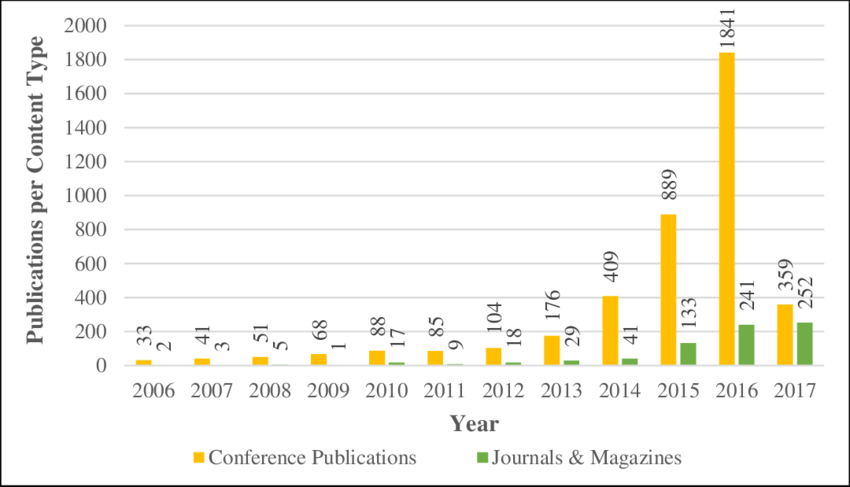
\includegraphics[scale=0.25]{pub_DL_IEEE.png}
%         \label{fig:pub_DL_IEEE}
%     \end{figure}
% \end{frame}

%% ---------------------------------------------------------------------------
% SECTION: Resultados
\section{Resultados}

\attachfilesetup{
    color = {1 0 0}
} 

\begin{frame}{Implementação dos algoritmos}
    Os algoritmos apresentados foram implementados com a ajuda dos seguintes softwares.
    \vspace{0.5cm}
    
    \begin{itemize}
        \item MATLAB\textregistered \  R2018a
        \item ITA Toolbox (plugin para MATLAB) \cite{ITA_Toolbox}
    \end{itemize}
    \vspace{0.5cm}

    São utilizadas três bases de dados para gerar as RIRSMs e AVCDs.
    \vspace{0.5cm}

    \begin{itemize}
        \item Base de amostras de voz anecóicas
        \item Base de RIRs - Aachen Impulse Response database
        \item Base de ruídos - MUSAN
    \end{itemize}
\end{frame}

\begin{frame}{Implementação dos algoritmos}
    Configurações das características desejadas.
    \vspace{1cm}

    \begin{table} [H]
        \centering
        \begin{tabular}{c|p{7cm}}
    
            \multicolumn{1}{c|}{\textbf{Parâmetro}} & \multicolumn{1}{c}{\textbf{Faixa}} \\
            \hline 
    
            $DRR_{alvo}$ (dB) & $-6 \le DRR_{alvo} \le 18 $ \\
            & \\
            $T60_{alvo}$ (s) & $T60_{org} - 1  \le T60_{alvo} \le T60_{org} + 1$ , onde o limite inferior de $T60_{alvo} = 0.2$ \\
            & \\
            $SNR_{alvo}$ & $3 \le SNR_{alvo} \le 20 $ \\
    
        \end{tabular}
    \end{table}
\end{frame}

%% ---------------------------------------------------------------------------
% RESULTADOS - DRR
\begin{frame}{Resultados - DRR}
    \begin{table} [H]
        \centering
        \label{tbl:da-drr}
        \begin{tabular}{c|c|c|c}
    
            \textbf{Exemplo} & 
            \textbf{Sala RIR} & 
            \textbf{Distância (m)} &
            \textbf{Amostra de Voz} \\
            \hline 
    
            D1 & lecture & 7.1 & H2-T2 \\
            D2 & booth & 1 & H2-T1 \\
            D3 & office & 2 & M2-T2 \\
    
        \end{tabular}
        \bigbreak
        \bigbreak
        \begin{tabular}{c|c|c|c|c}
    
            \textbf{Exemplo} & 
            \textbf{$DRR_{org}$ (dB)} & 
            \textbf{$DRR_{alvo}$ (dB)} &
            \textbf{$DRR_{res}$ (dB)} & 
            \textbf{$\rho_{DRR}$ (\%)} \\
            \hline 
    
            D1 & -4,5 & 10 & 10 & 0 \\
            D2 & 4,7 & -2 & -2 & 0 \\
            D3 & 0,5 & 18 & 18 & 0 \\
    
        \end{tabular}
        \vspace{0.5cm}

        $\rho_{DRR} = |DRR_{res} - DRR_{alvo}|/DRR_{alvo}$
    \end{table}
\end{frame}

\begin{frame}{Resultados - DRR}
    \textbf{Experimento empírico}: sensação subjetiva de “distância”, ordenado de mais para menos distante.
    \vspace{1cm}
    
    \begin{table} [H]
        \centering
        \begin{tabular}{c|c|c|c|c}
    
            \textbf{Exemplo} & 
            \textbf{$DRR_{org}$ (dB)} & 
            \textbf{$DRR_{res}$ (dB)} & 
            \textbf{Comparação} &
            \textbf{Ordem} \\
            \hline 
    
            D1 & -4,5 & 10 & original & 2 \\
            D2 & 4,7 & -2 & simulado & 1 \\
            D3 & 0,5 & 18 & original & 3 \\
    
        \end{tabular}
    \end{table}
\end{frame}

\begin{frame}{Exemplo D1}
    \begin{columns}
        \column{.6\textwidth}
        \begin{figure}
            \begin{subfigure}{\textwidth}
                \centering
                \notextattachfile{\scriptsize RIR Original}
                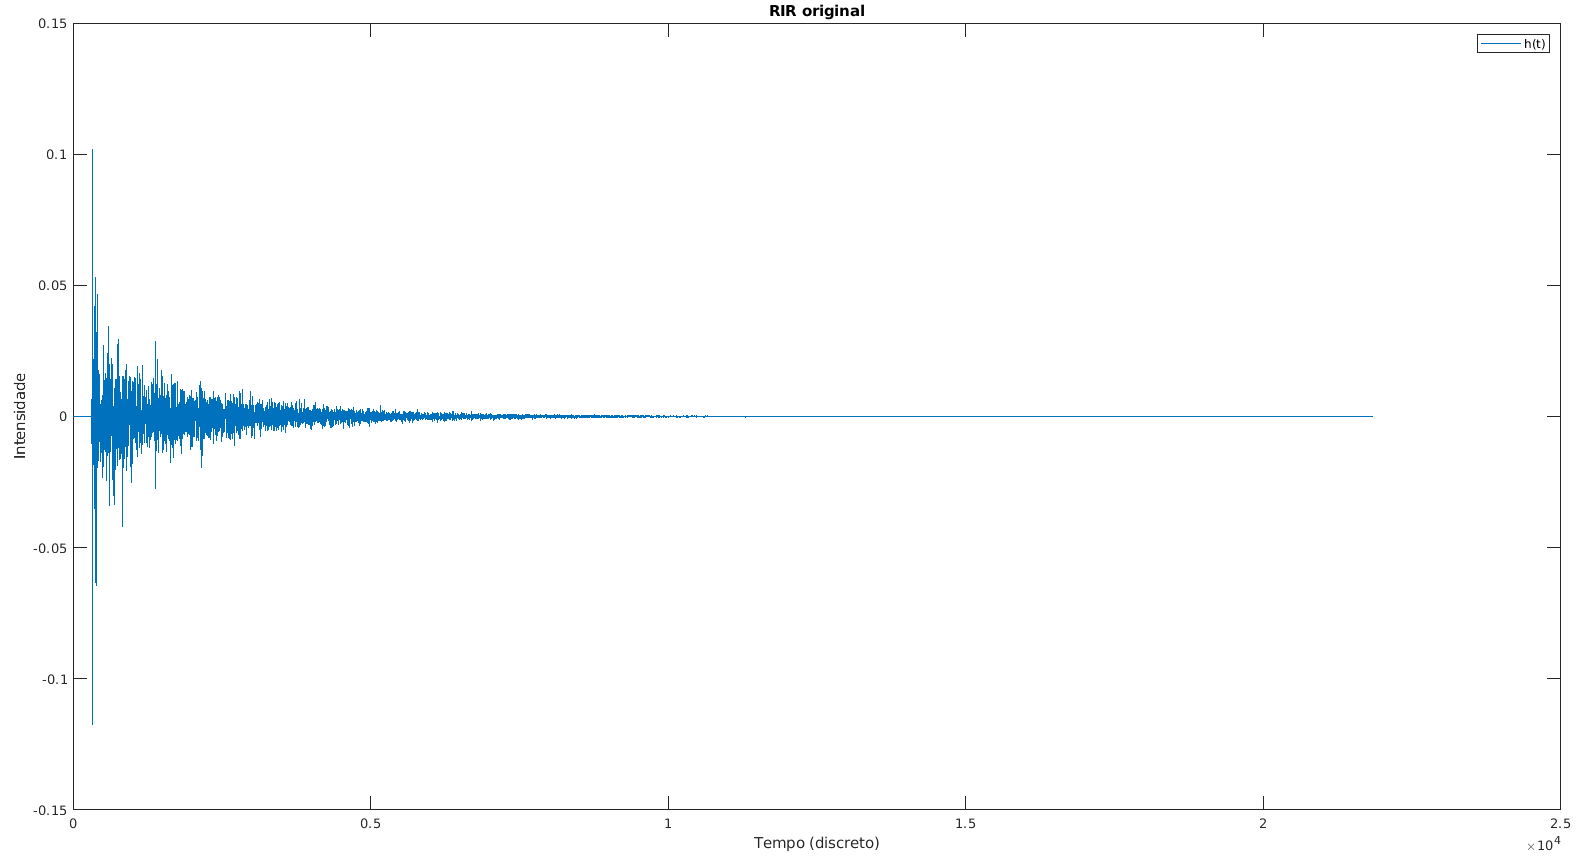
\includegraphics[scale=0.115]{rir-og-d1.png}
            \end{subfigure}
            \begin{subfigure}{\textwidth}
                \centering
                \notextattachfile{\scriptsize RIR Simulada}
                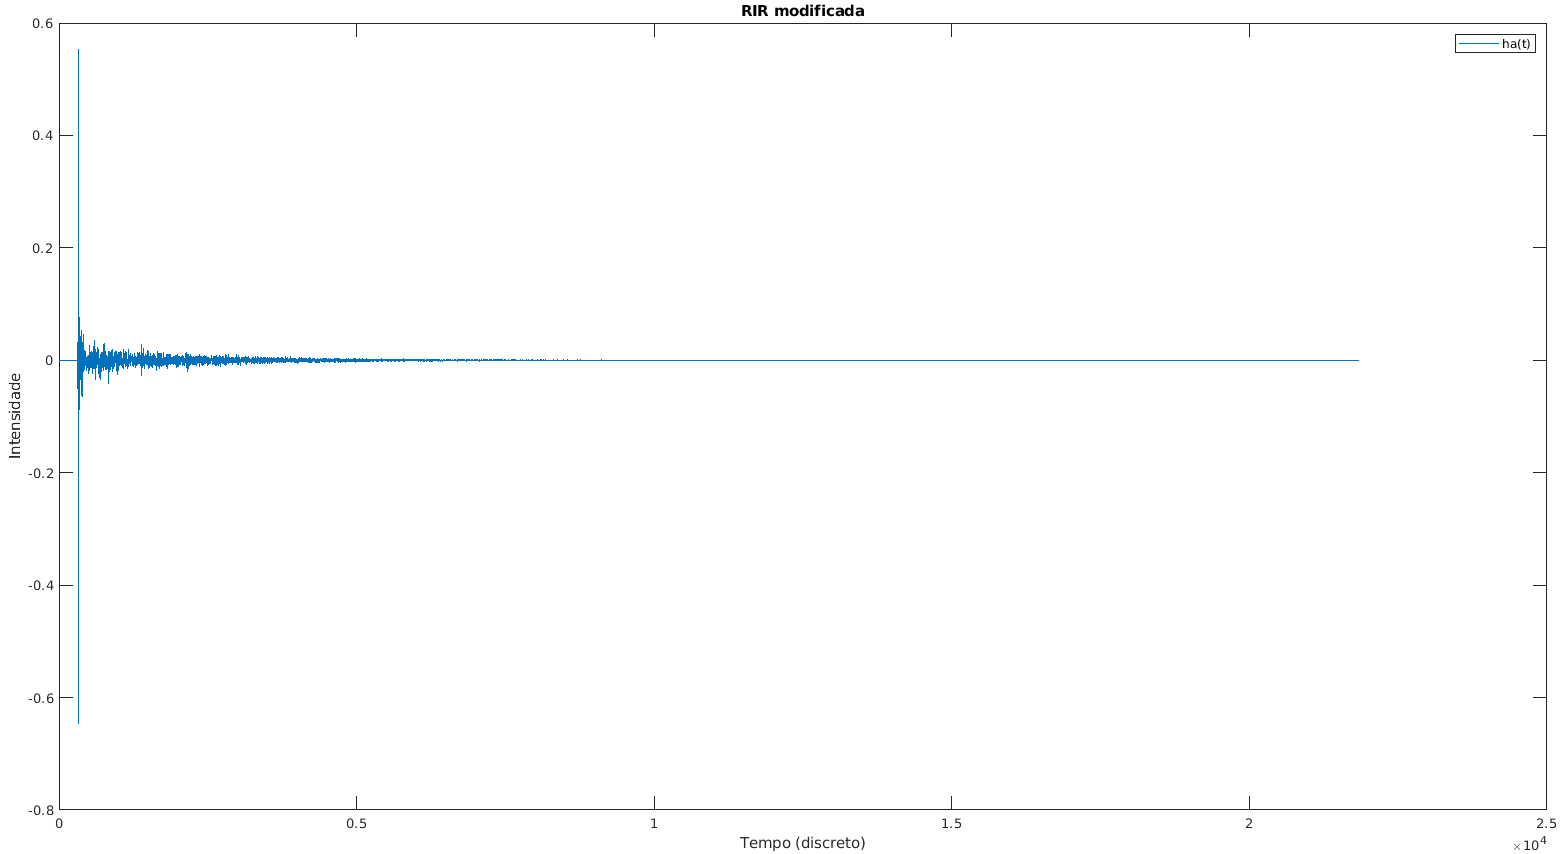
\includegraphics[scale=0.115]{rir-aug-d1.png}
            \end{subfigure}
        \end{figure}
    \end{columns}
        
\end{frame}

\begin{frame}{Exemplo D1}
    \begin{columns}
        \column{0.5\textwidth}
        \begin{figure}
            \begin{subfigure}{\textwidth}
                \centering
                \textattachfile{audios/voice-og-d1.wav}{\scriptsize amostra de voz original}
                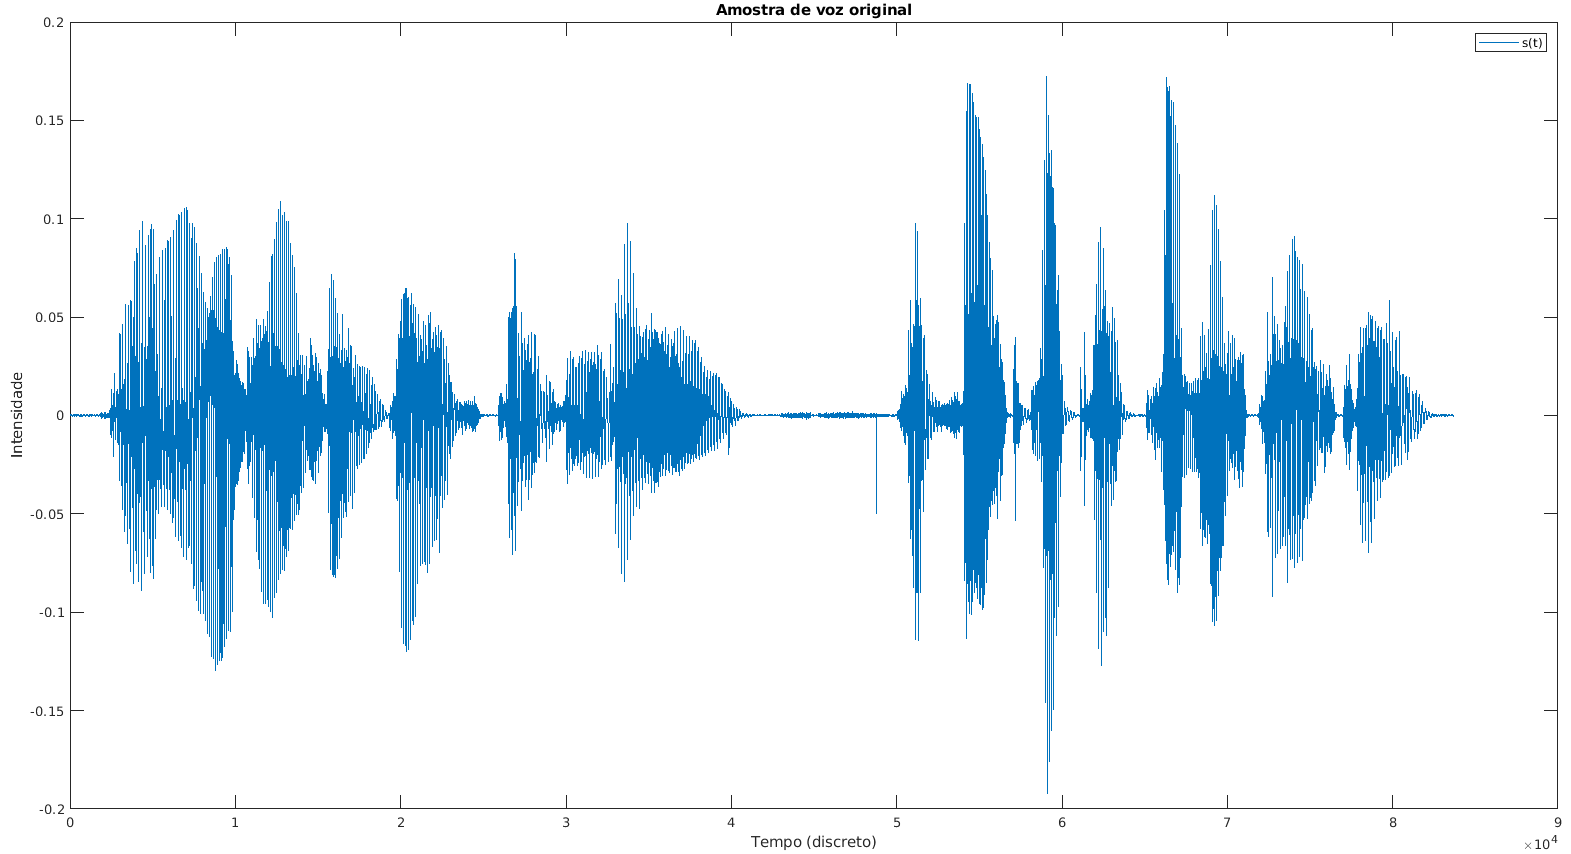
\includegraphics[scale=0.105]{voice-og-d1.png}
            \end{subfigure}
        \end{figure}

        \column{0.5\textwidth}
        \begin{figure}
            \begin{subfigure}{\textwidth}
                \centering
                \textattachfile{audios/voice-aug-riro-d1.wav}{\footnotesize amostra de voz reverberada - RIRO}
                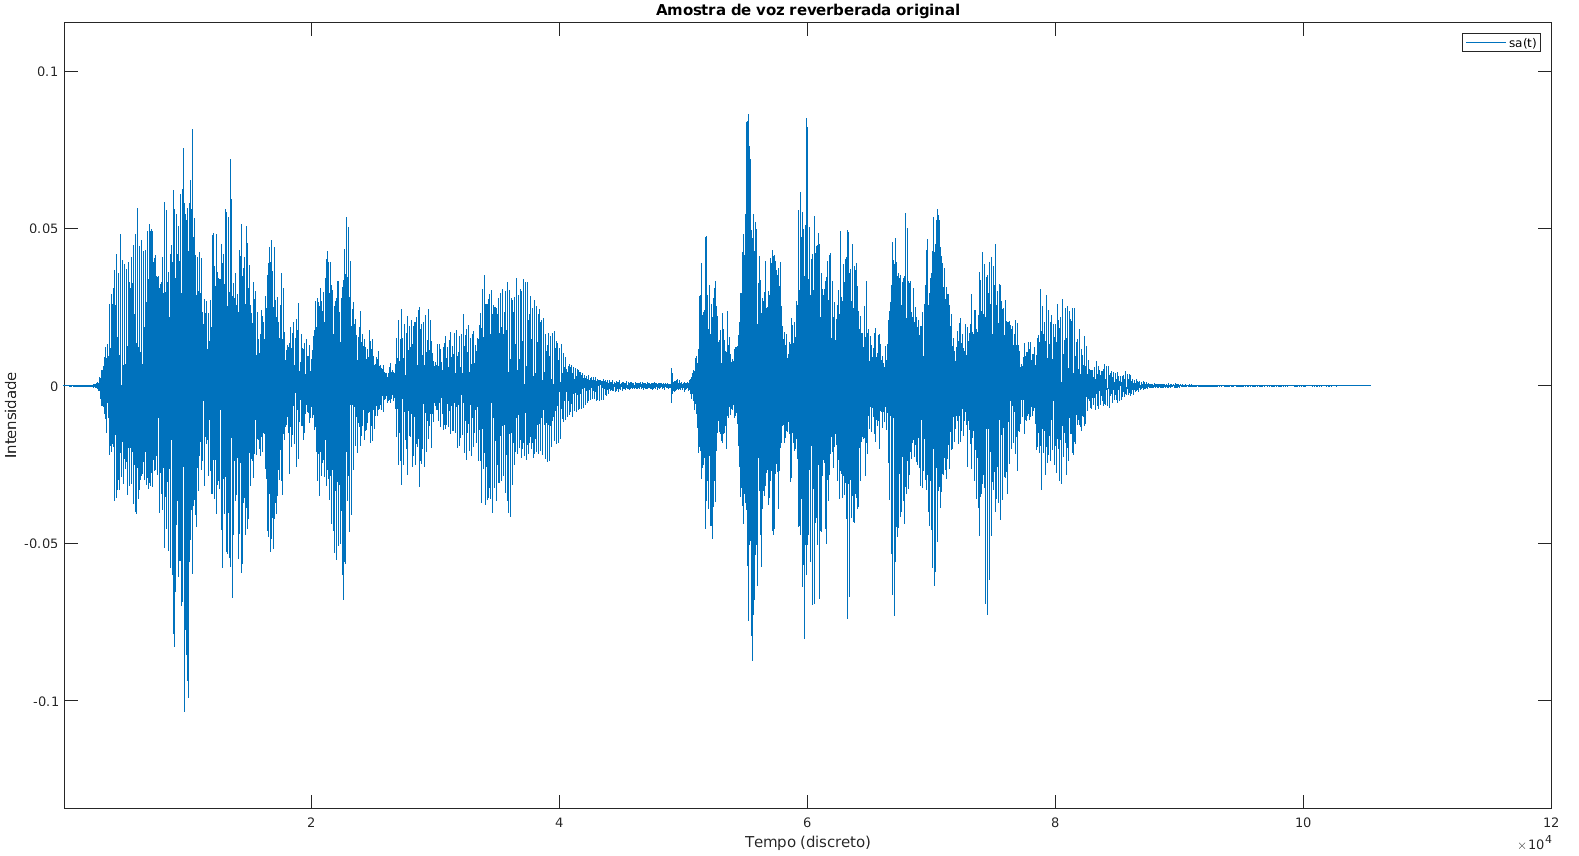
\includegraphics[scale=0.105]{voice-aug-riro-d1.png}
            \end{subfigure}
            \begin{subfigure}{\textwidth}
                \centering
                \textattachfile{audios/voice-aug-d1.wav}{\footnotesize amostra de voz reverberada - RIRSM}
                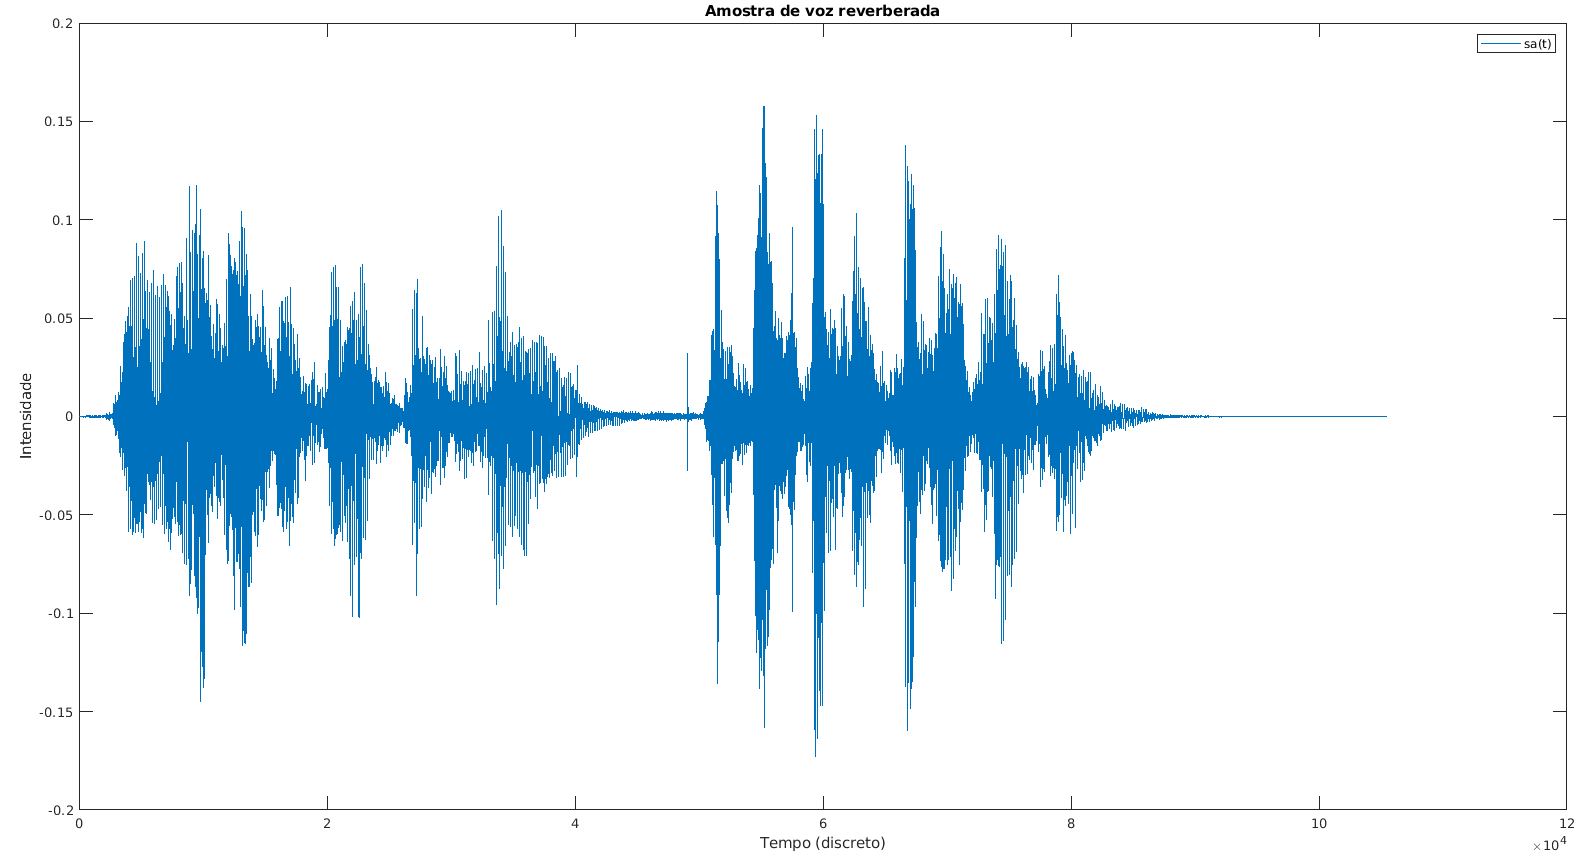
\includegraphics[scale=0.105]{voice-aug-d1.png}
            \end{subfigure}
        \end{figure}
    \end{columns}
\end{frame}

\begin{frame}{Exemplo D2}
    \begin{columns}
        \column{.6\textwidth}
        \begin{figure}
            \begin{subfigure}{\textwidth}
                \centering
                \notextattachfile{\scriptsize RIR Original}
                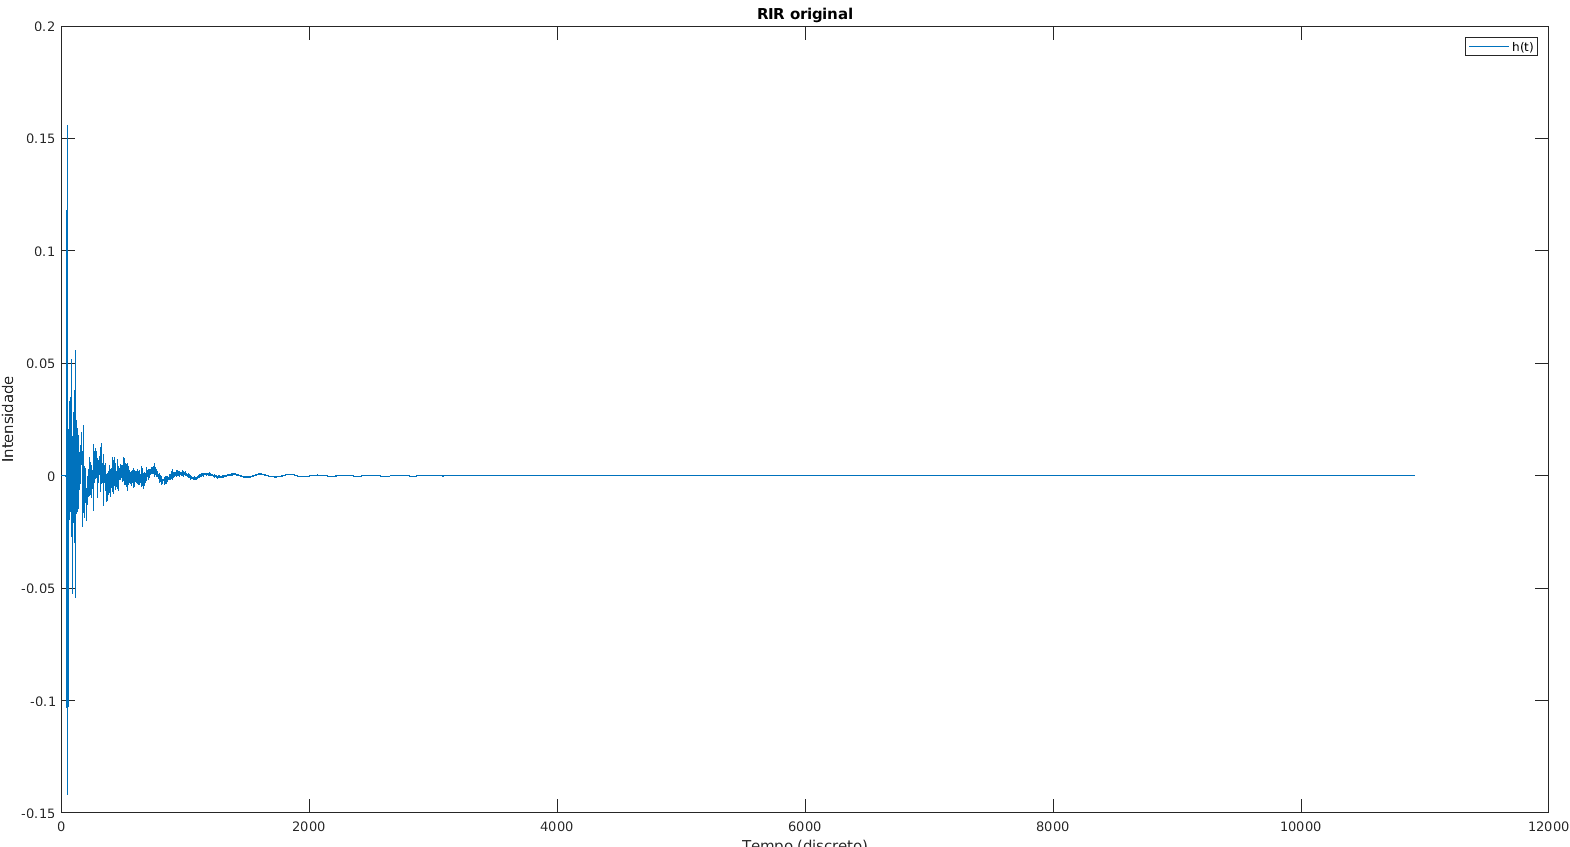
\includegraphics[scale=0.115]{rir-og-d2.png}
            \end{subfigure}
            \begin{subfigure}{\textwidth}
                \centering
                \notextattachfile{\scriptsize RIR Simulada}
                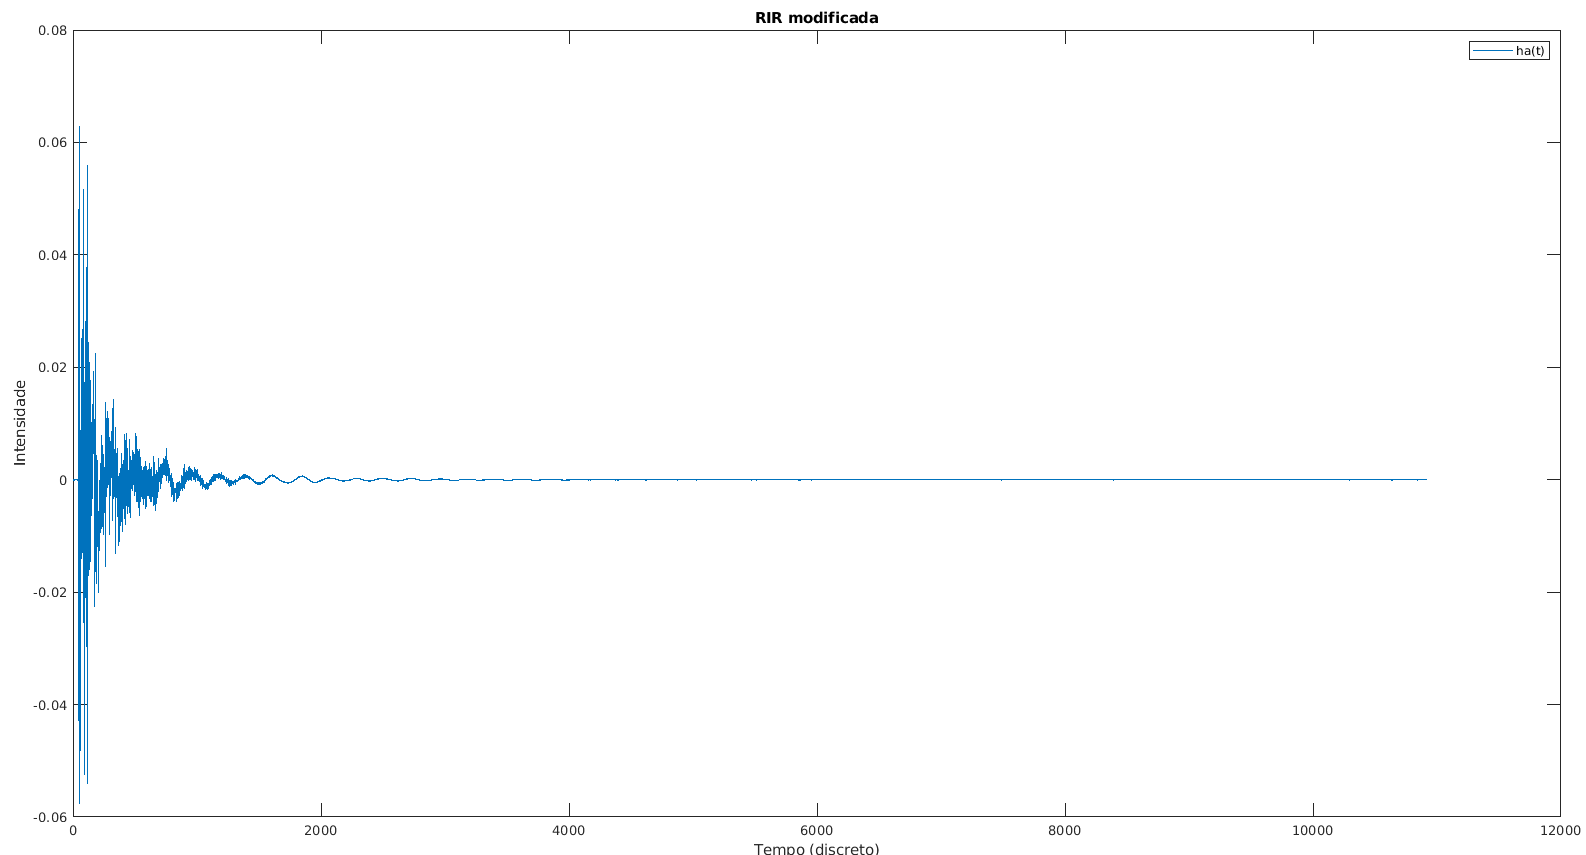
\includegraphics[scale=0.115]{rir-aug-d2.png}
            \end{subfigure}
        \end{figure}
    \end{columns}
        
\end{frame}

\begin{frame}{Exemplo D2}
    \begin{columns}
        \column{0.5\textwidth}
        \begin{figure}
            \begin{subfigure}{\textwidth}
                \centering
                \textattachfile{audios/voice-og-d2.wav}{\scriptsize amostra de voz original}
                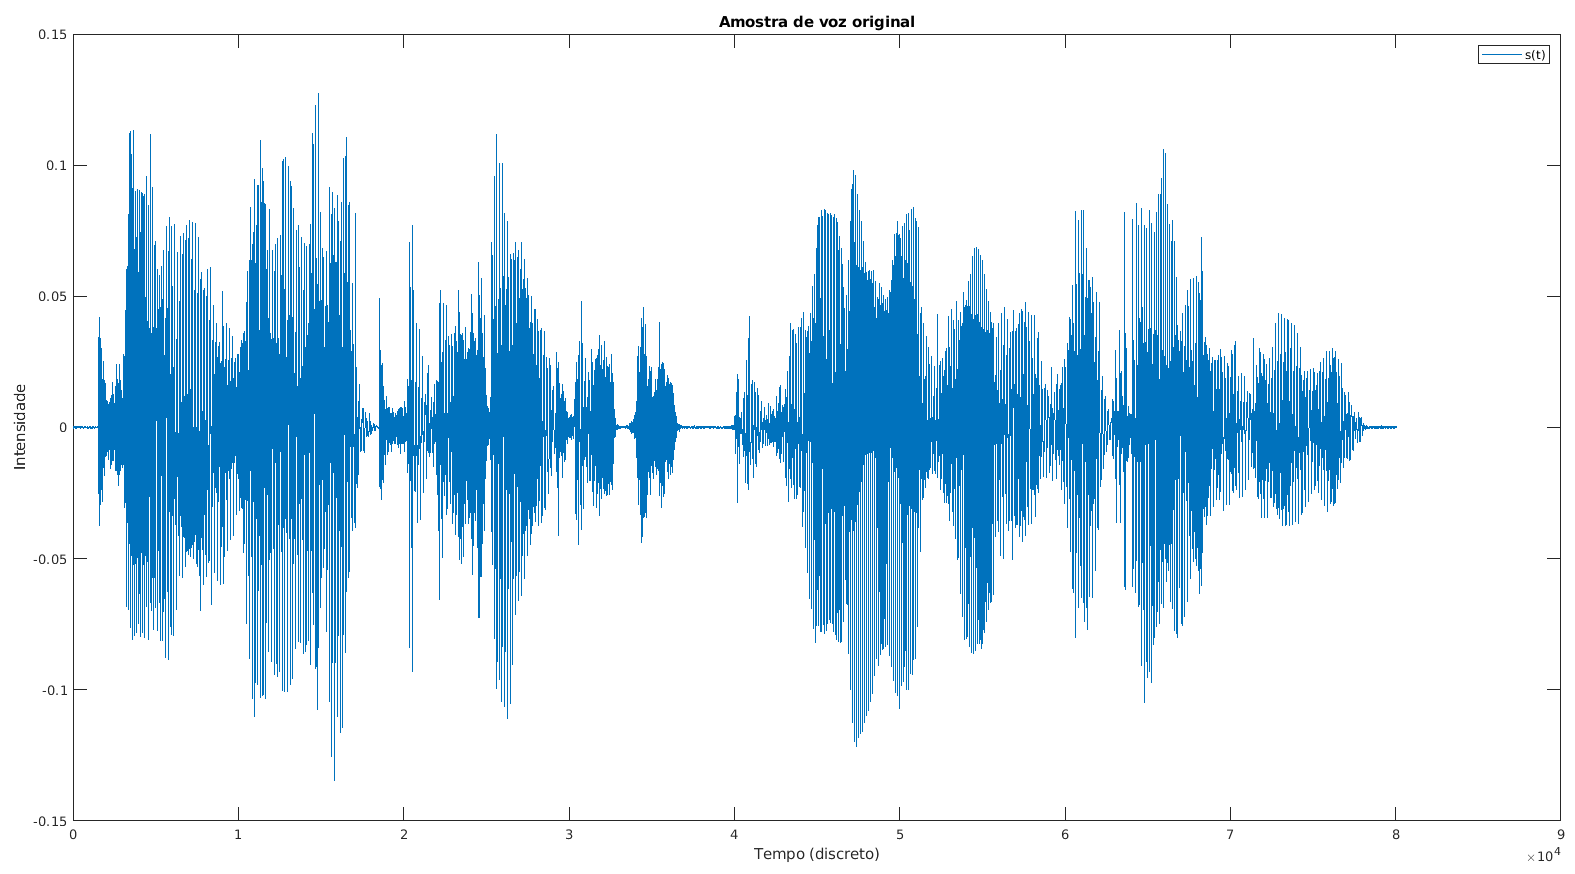
\includegraphics[scale=0.105]{voice-og-d2.png}
            \end{subfigure}
        \end{figure}

        \column{0.5\textwidth}
        \begin{figure}
            \begin{subfigure}{\textwidth}
                \centering
                \textattachfile{audios/voice-aug-riro-d2.wav}{\footnotesize amostra de voz reverberada - RIRO}
                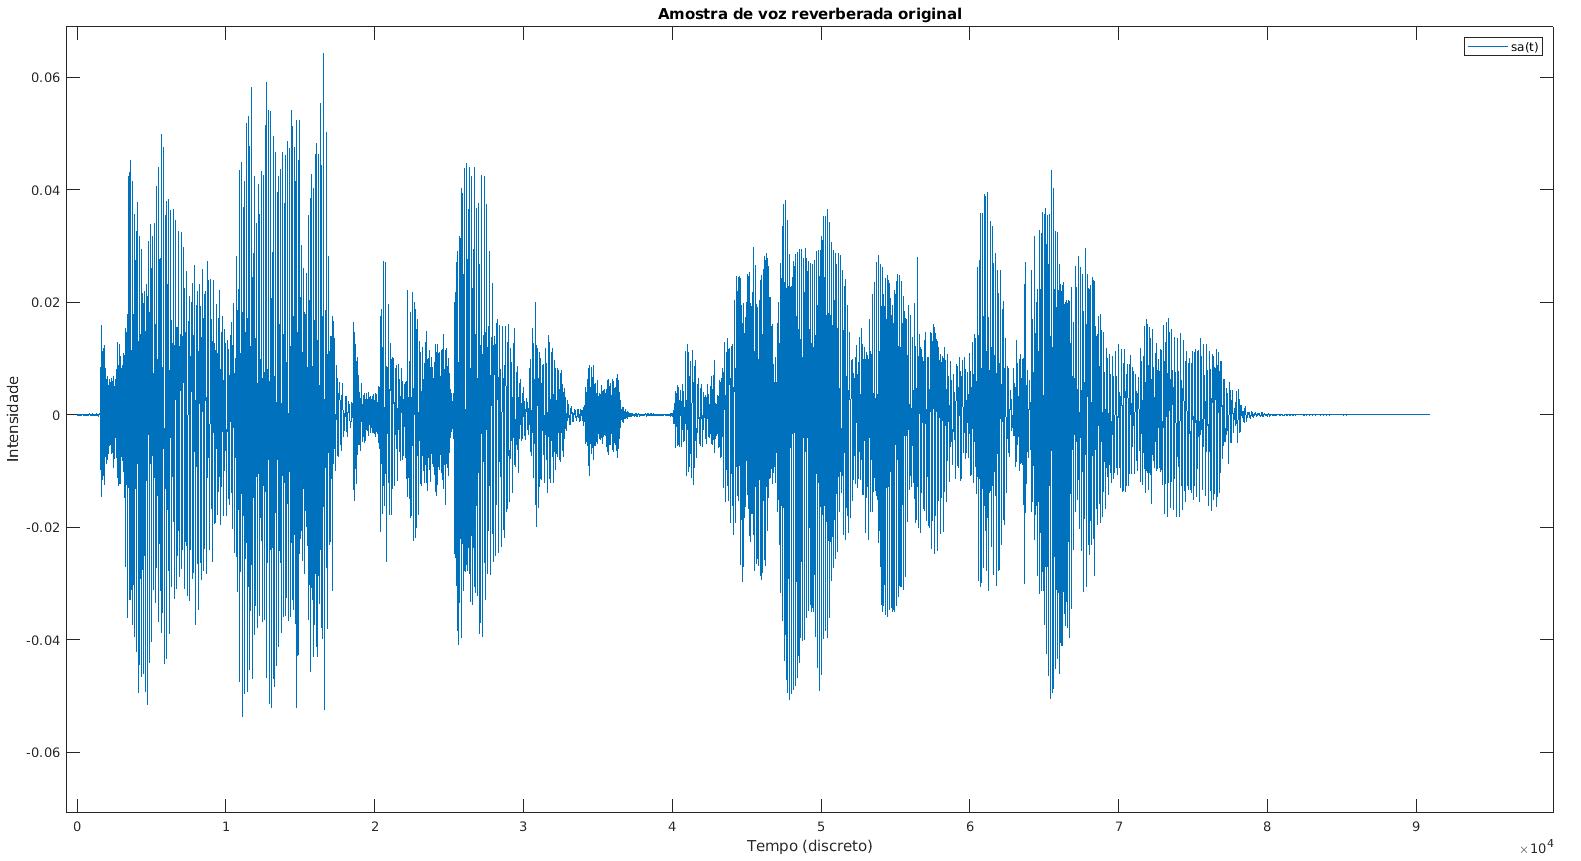
\includegraphics[scale=0.105]{voice-aug-riro-d2.png}
            \end{subfigure}
            \begin{subfigure}{\textwidth}
                \centering
                \textattachfile{audios/voice-aug-d2.wav}{\footnotesize amostra de voz reverberada - RIRSM}
                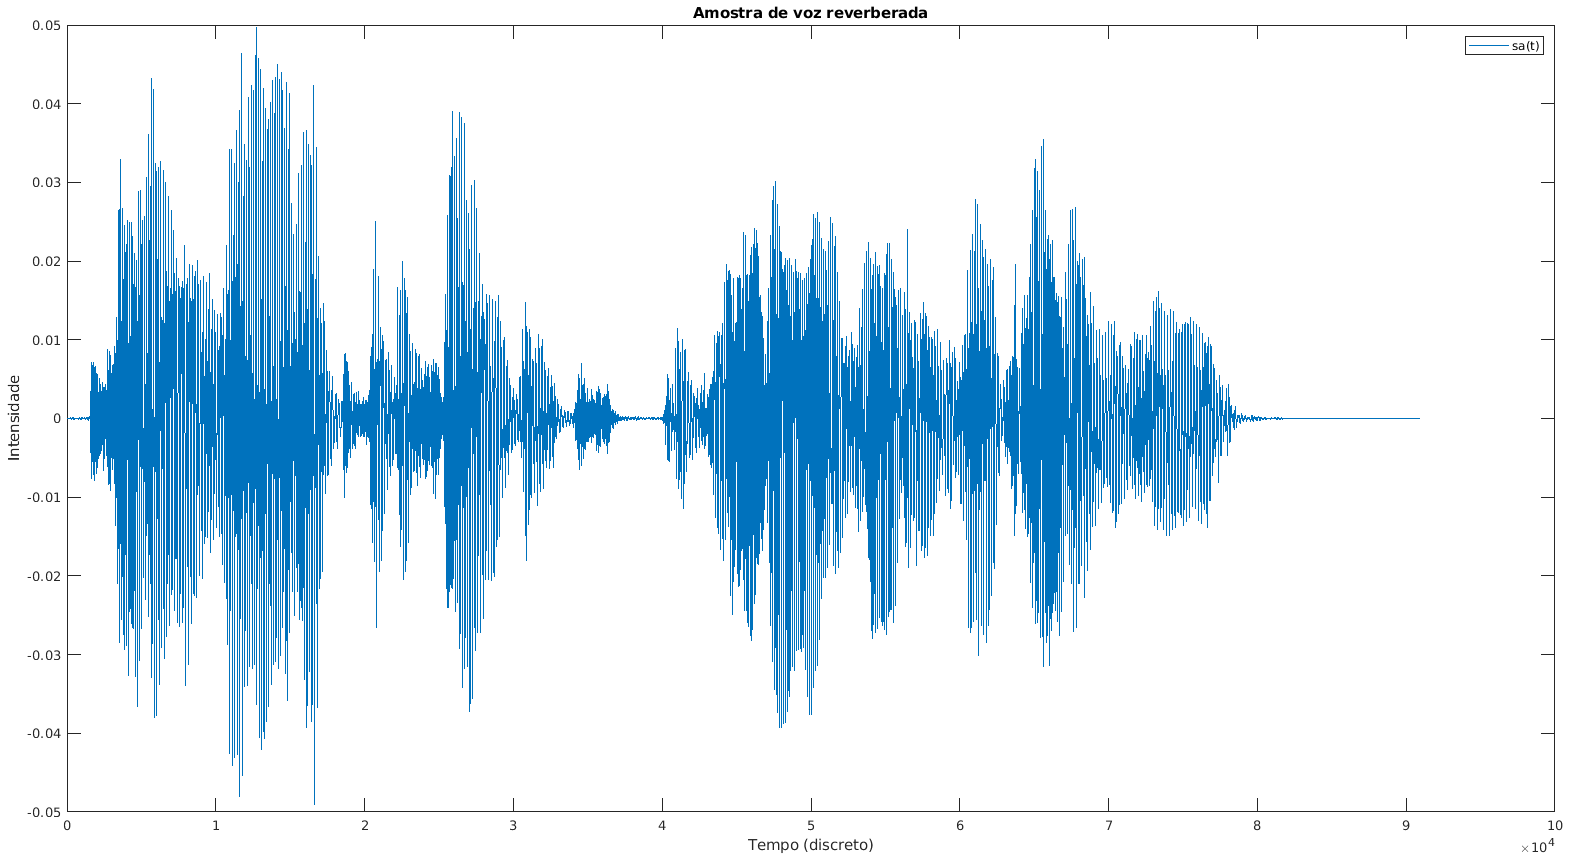
\includegraphics[scale=0.105]{voice-aug-d2.png}
            \end{subfigure}
        \end{figure}
    \end{columns}
\end{frame}

%% ---------------------------------------------------------------------------
% RESULTADOS - T60

\begin{frame}{Resultados - T60}
    \begin{table} [H]
        \centering
        \begin{tabular}{c|c|c|c}
    
            \textbf{Exemplo} & 
            \textbf{Sala RIR} & 
            \textbf{Distância (m)} &
            \textbf{Amostra de Voz} \\
            \hline 
    
            T1 & lecture & 7.1 & M2-T1 \\
            T2 & booth & 1 & H1-T2 \\
            T3 & office & 2 & H2-T2 \\
    
        \end{tabular}
        \bigbreak
        \bigbreak
        \begin{tabular}{c|c|c|c|c}
    
            \textbf{Exemplo} & 
            \textbf{$T60_{org}$ (s)} & 
            \textbf{$T60_{alvo}$ (s)} &
            \textbf{$T60_{res}$ (s)} & 
            \textbf{$\rho_{T60}$ (\%)} \\
            \hline 
    
            T1 & 1,38 & 1,15 & 1,01 & 12.1 \\
            T2 & 1,01 & 1,88 & 1,89 & 0,5 \\
            T3 & 0,75 & 0,61 & 0,60 & 1,6 \\
    
        \end{tabular}
        \vspace{0.5cm}

        $\rho_{T60} = |T60_{res} - T60_{alvo}|/T60_{alvo}$
    \end{table}
\end{frame}

\begin{frame}{Resultados - T60}
    \textbf{Experimento empírico}: sensação subjetiva de “eco”, ordenado de mais para menos ecoante.
    \vspace{1cm}

    \begin{table} [H]
        \centering
        \begin{tabular}{c|c|c|c|c}
    
            \textbf{Exemplo} & 
            \textbf{$T60_{org}$ (s)} & 
            \textbf{$T60_{res}$ (s)} & 
            \textbf{Comparação} &
            \textbf{Ordem} \\
            \hline 
    
            T1 & 1,38 & 1,01 & original & 2 \\
            T2 & 1,01 & 1,89 & simulado & 1 \\
            T3 & 0,75 & 0,60 & original & 3 \\
    
        \end{tabular}
    \end{table}
\end{frame}

\begin{frame}{Exemplo T1}
    \begin{columns}
        \column{.6\textwidth}
        \begin{figure}
            \begin{subfigure}{\textwidth}
                \centering
                \notextattachfile{\scriptsize RIR Original}
                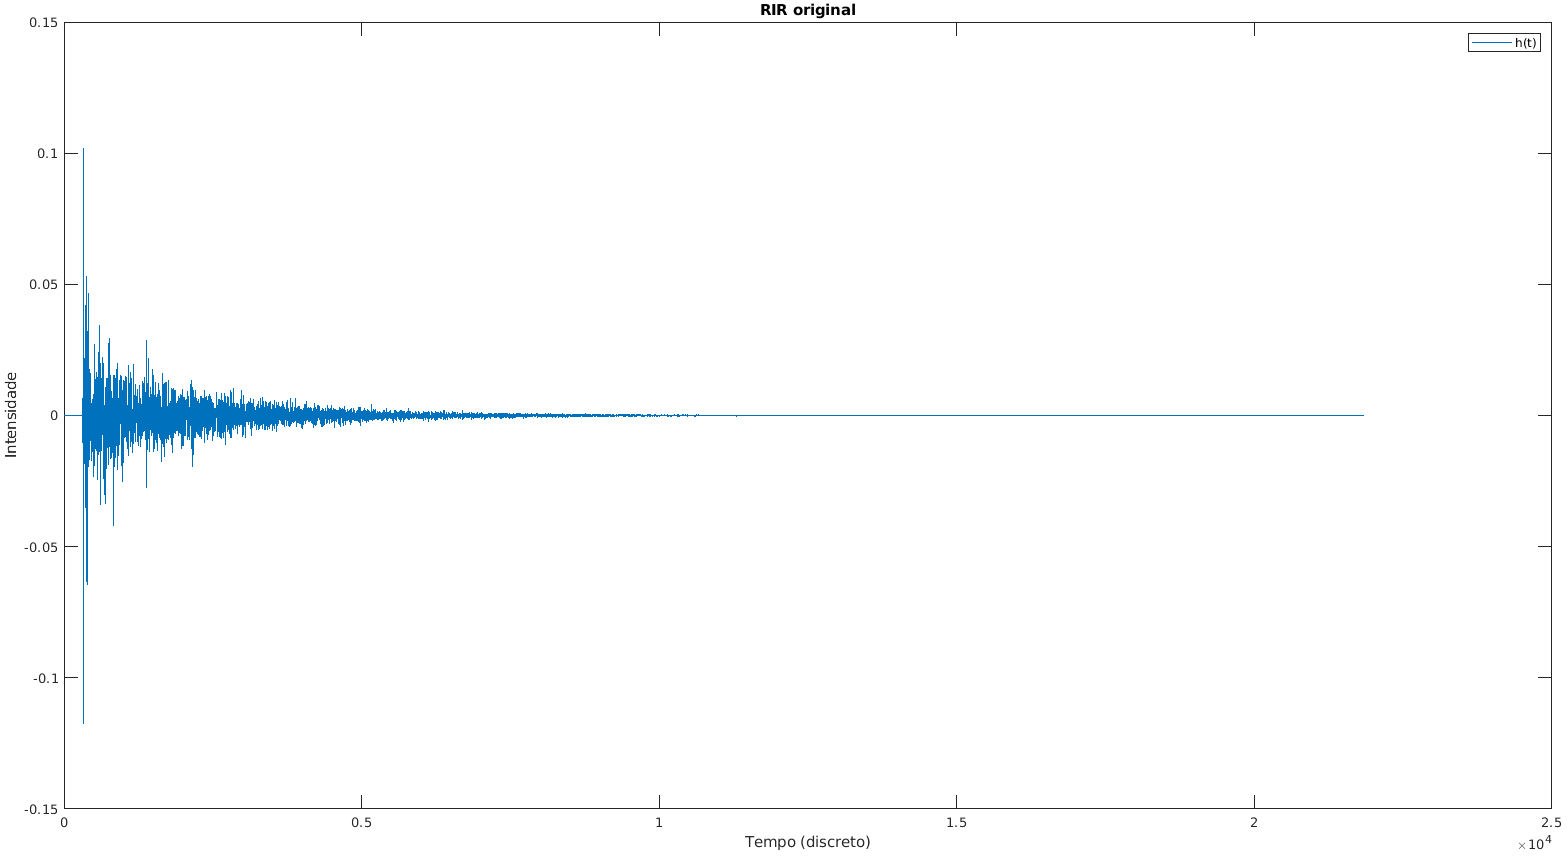
\includegraphics[scale=0.115]{rir-og-t1.png}
            \end{subfigure}
            \begin{subfigure}{\textwidth}
                \centering
                \notextattachfile{\scriptsize RIR Simulada}
                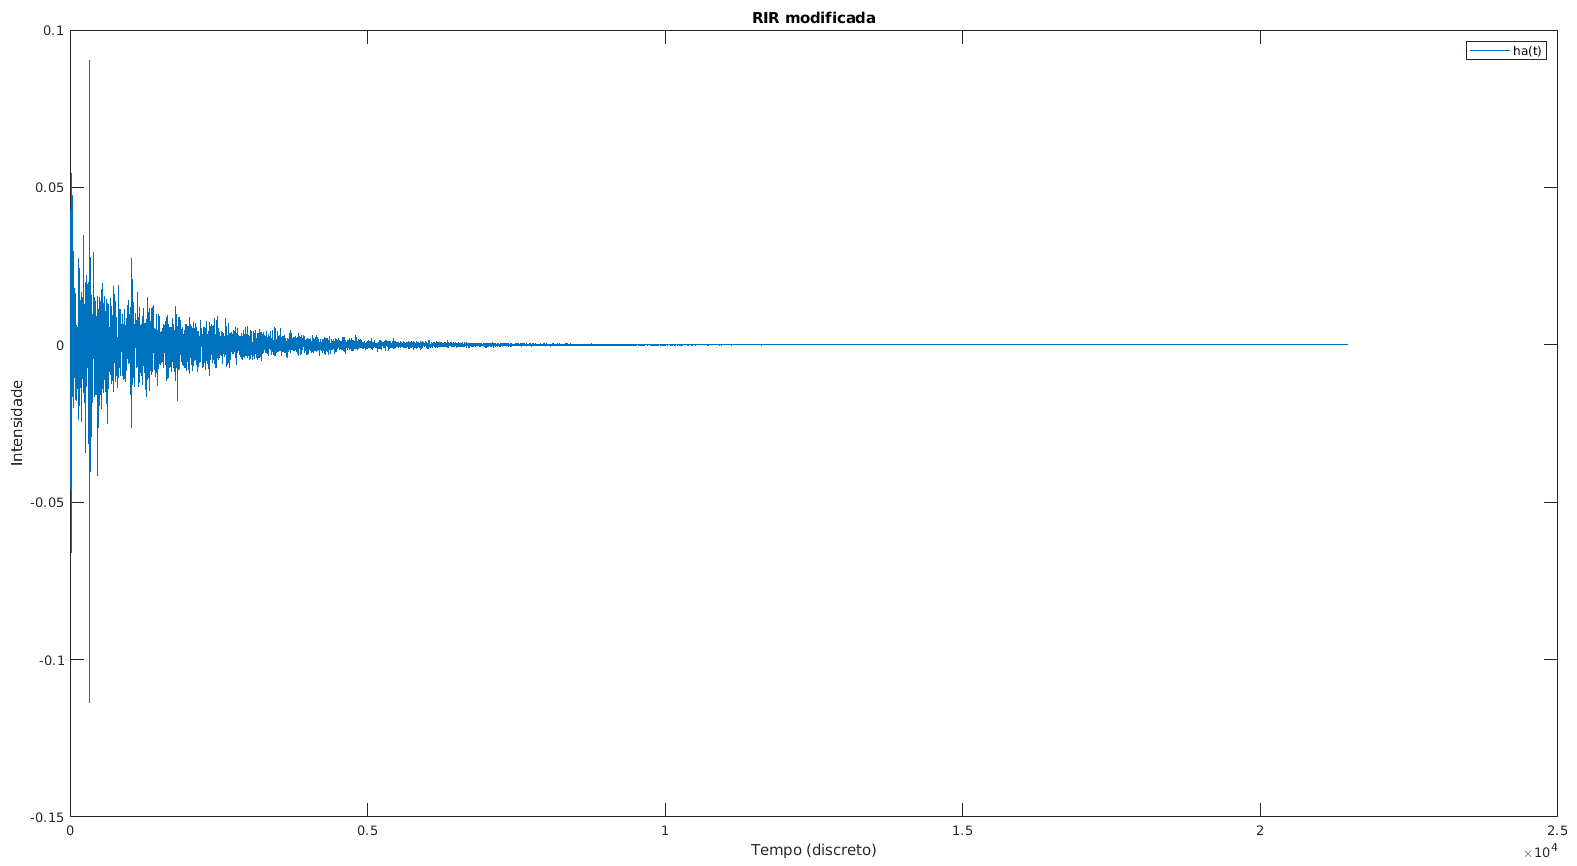
\includegraphics[scale=0.115]{rir-aug-t1.png}
            \end{subfigure}
        \end{figure}
    \end{columns}
        
\end{frame}

\begin{frame}{Exemplo T1}
    \begin{columns}
        \column{0.5\textwidth}
        \begin{figure}
            \begin{subfigure}{\textwidth}
                \centering
                \textattachfile{audios/voice-og-t1.wav}{\scriptsize amostra de voz original}
                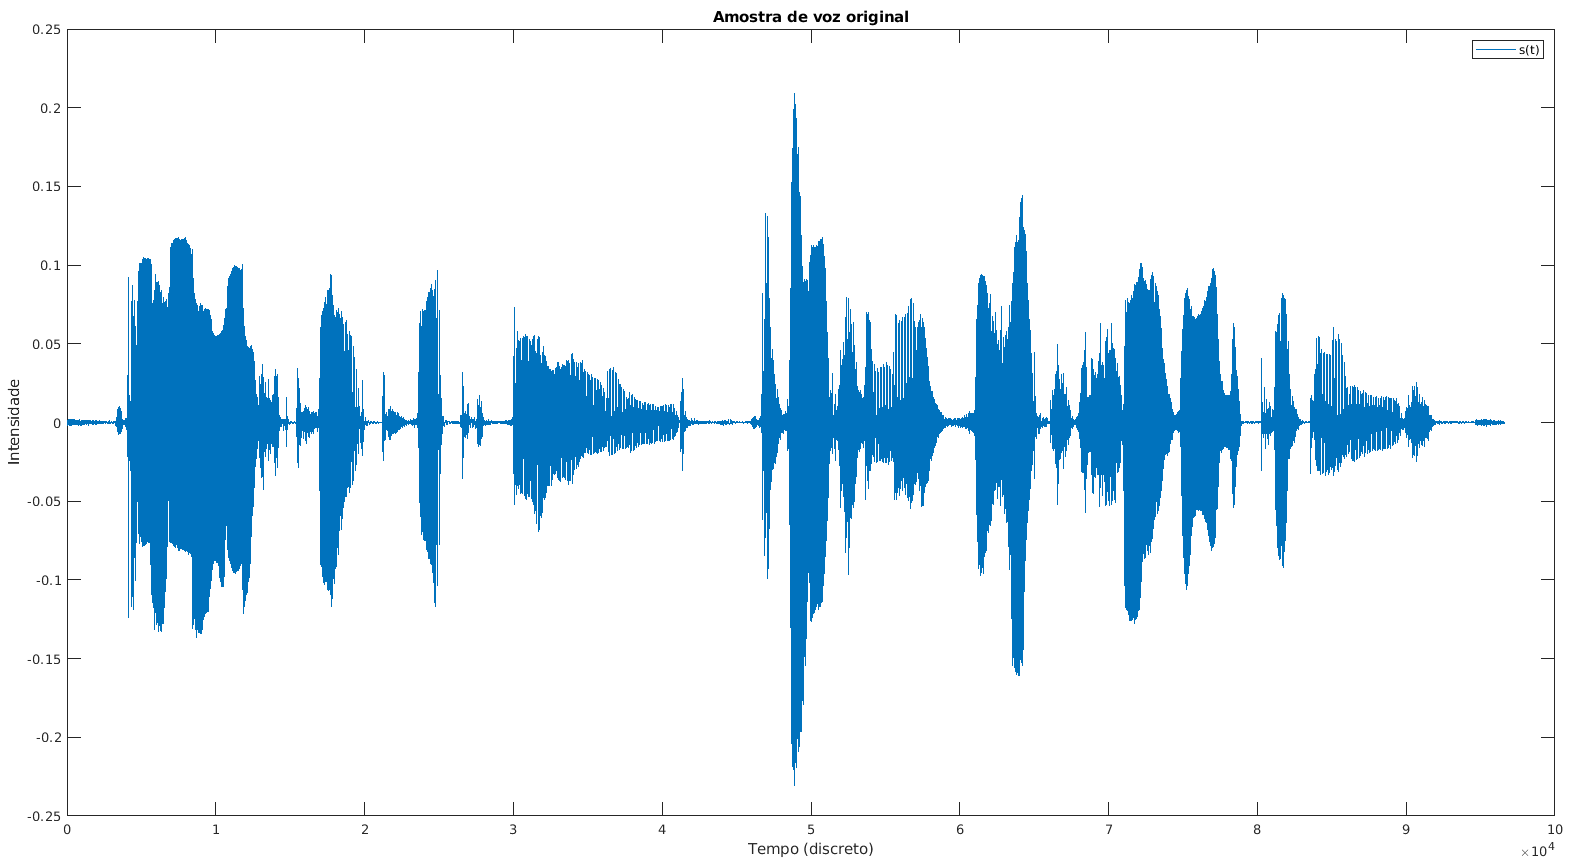
\includegraphics[scale=0.105]{voice-og-t1.png}
            \end{subfigure}
        \end{figure}

        \column{0.5\textwidth}
        \begin{figure}
            \begin{subfigure}{\textwidth}
                \centering
                \textattachfile{audios/voice-aug-riro-t1.wav}{\footnotesize amostra de voz reverberada - RIRO}
                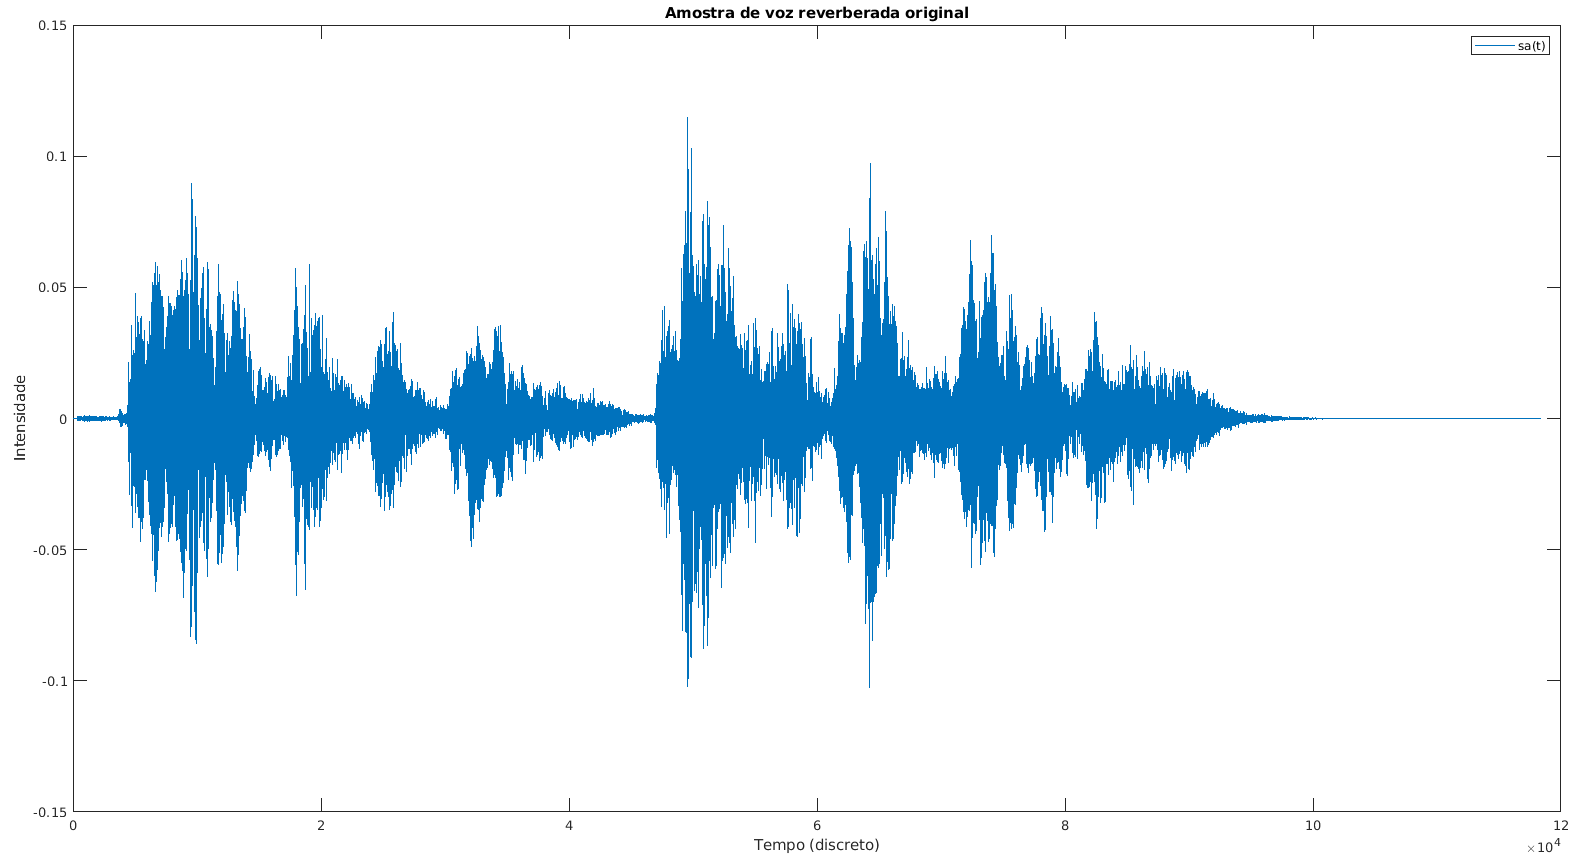
\includegraphics[scale=0.105]{voice-aug-riro-t1.png}
            \end{subfigure}
            \begin{subfigure}{\textwidth}
                \centering
                \textattachfile{audios/voice-aug-t1.wav}{\footnotesize amostra de voz reverberada - RIRSM}
                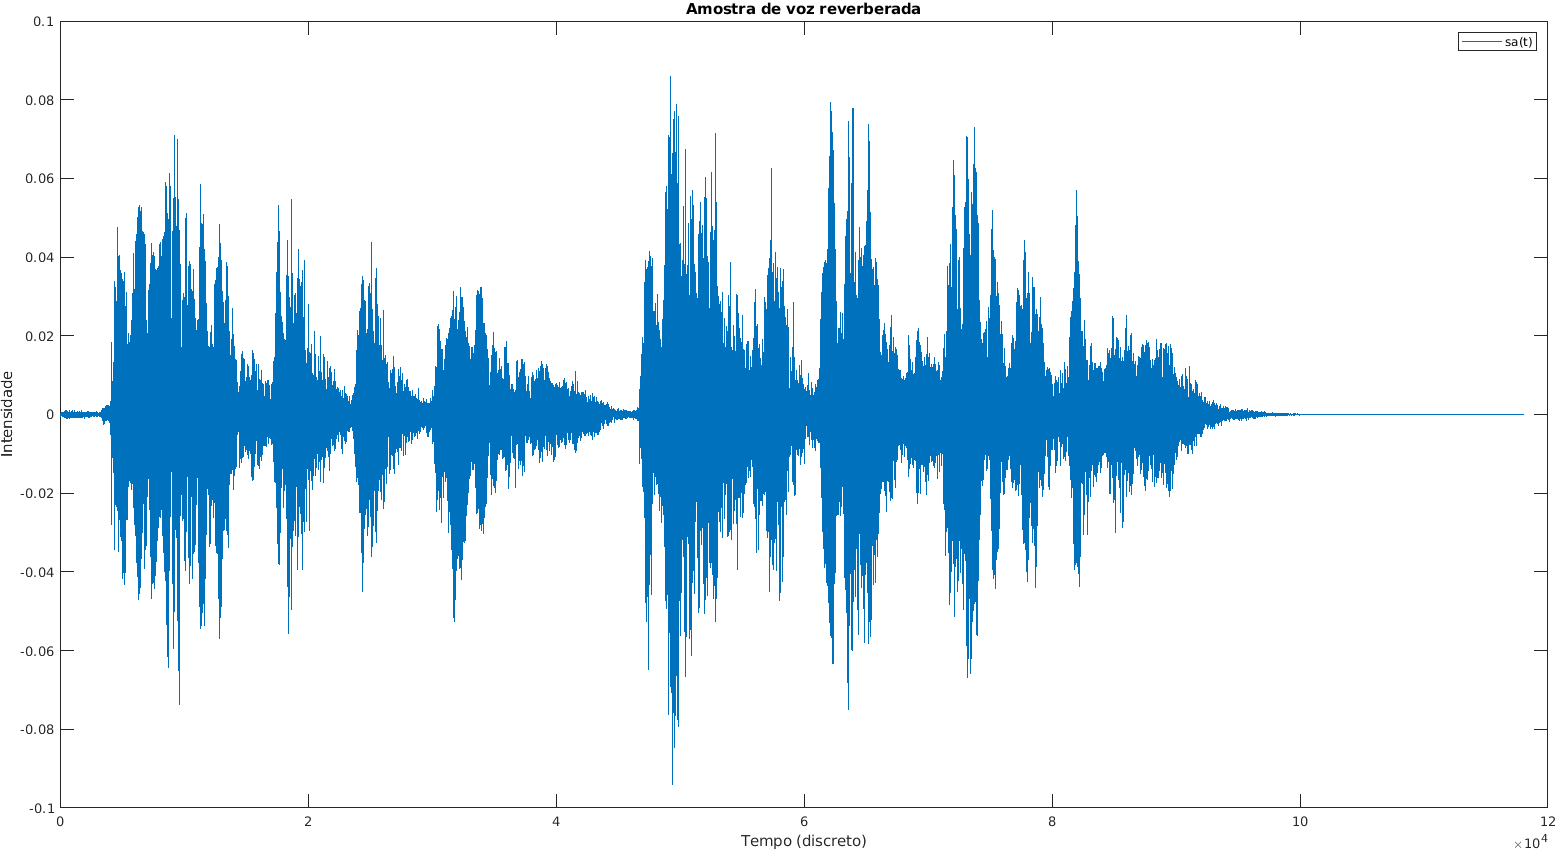
\includegraphics[scale=0.105]{voice-aug-t1.png}
            \end{subfigure}
        \end{figure}
    \end{columns}
\end{frame}

\begin{frame}{Exemplo T2}
    \begin{columns}
        \column{.6\textwidth}
        \begin{figure}
            \begin{subfigure}{\textwidth}
                \centering
                \notextattachfile{\scriptsize RIR Original}
                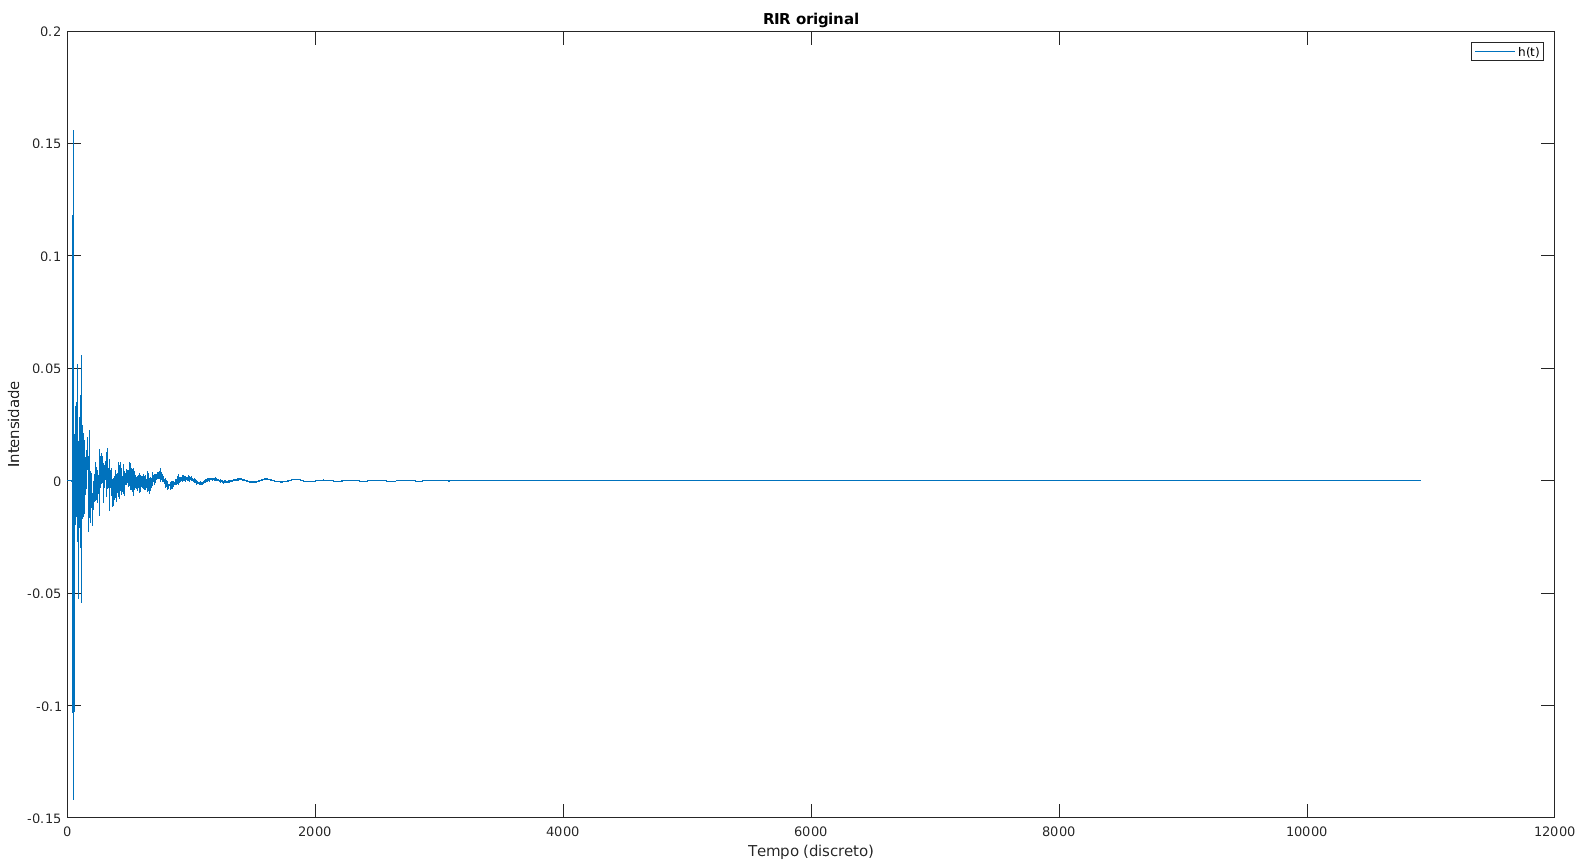
\includegraphics[scale=0.115]{rir-og-t2.png}
            \end{subfigure}
            \begin{subfigure}{\textwidth}
                \centering
                \notextattachfile{\scriptsize RIR Simulada}
                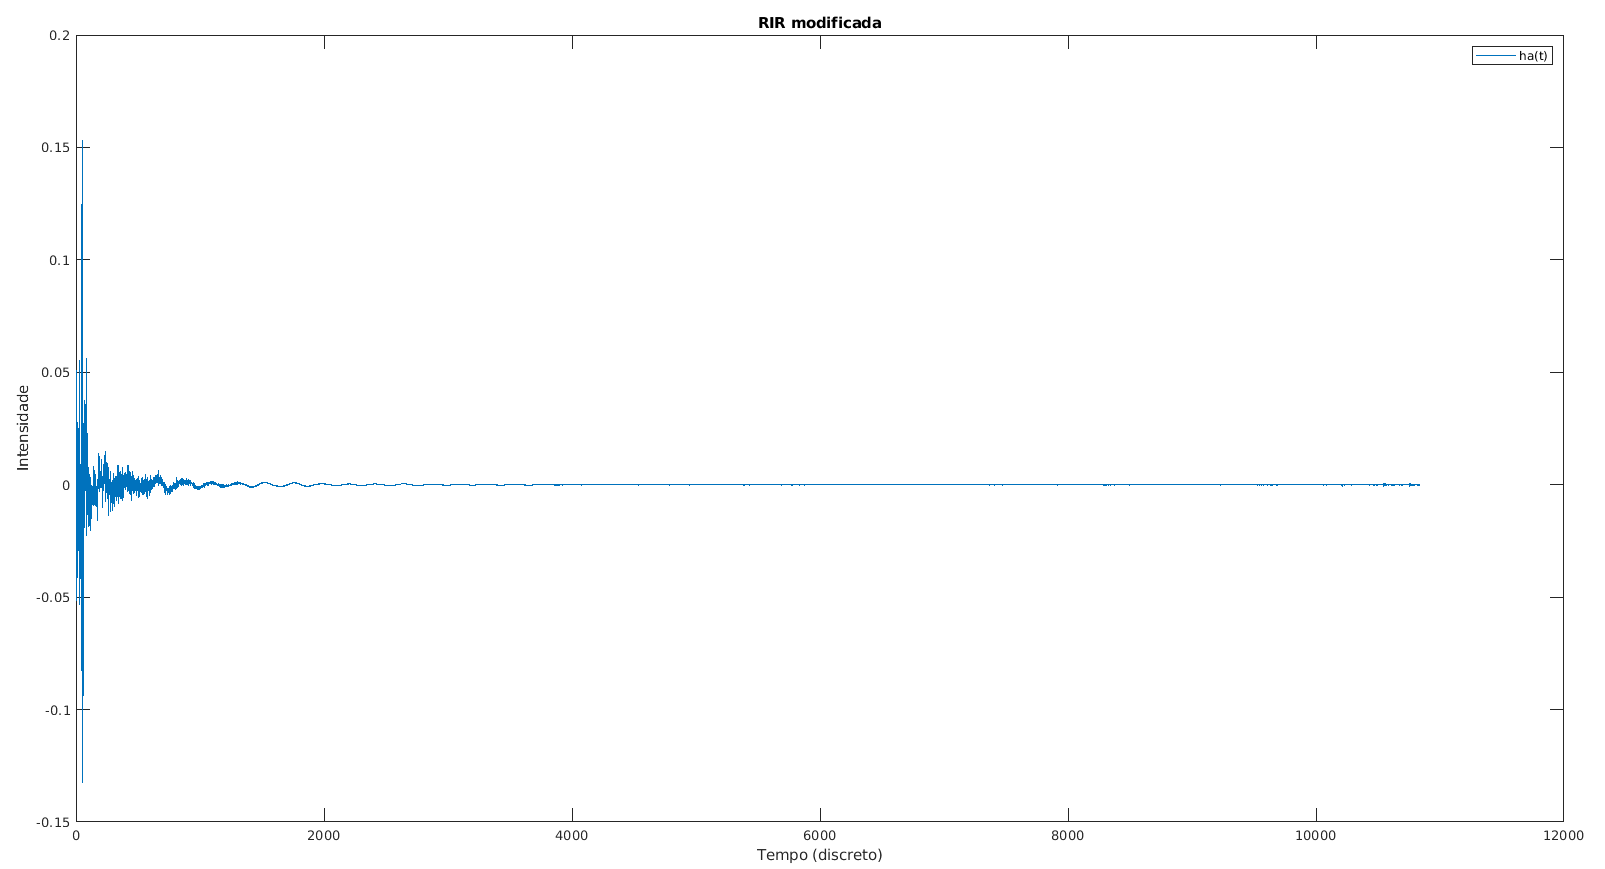
\includegraphics[scale=0.115]{rir-aug-t2.png}
            \end{subfigure}
        \end{figure}
    \end{columns}
        
\end{frame}

\begin{frame}{Exemplo T2}
    \begin{columns}
        \column{0.5\textwidth}
        \begin{figure}
            \begin{subfigure}{\textwidth}
                \centering
                \textattachfile{audios/voice-og-t2.wav}{\scriptsize amostra de voz original}
                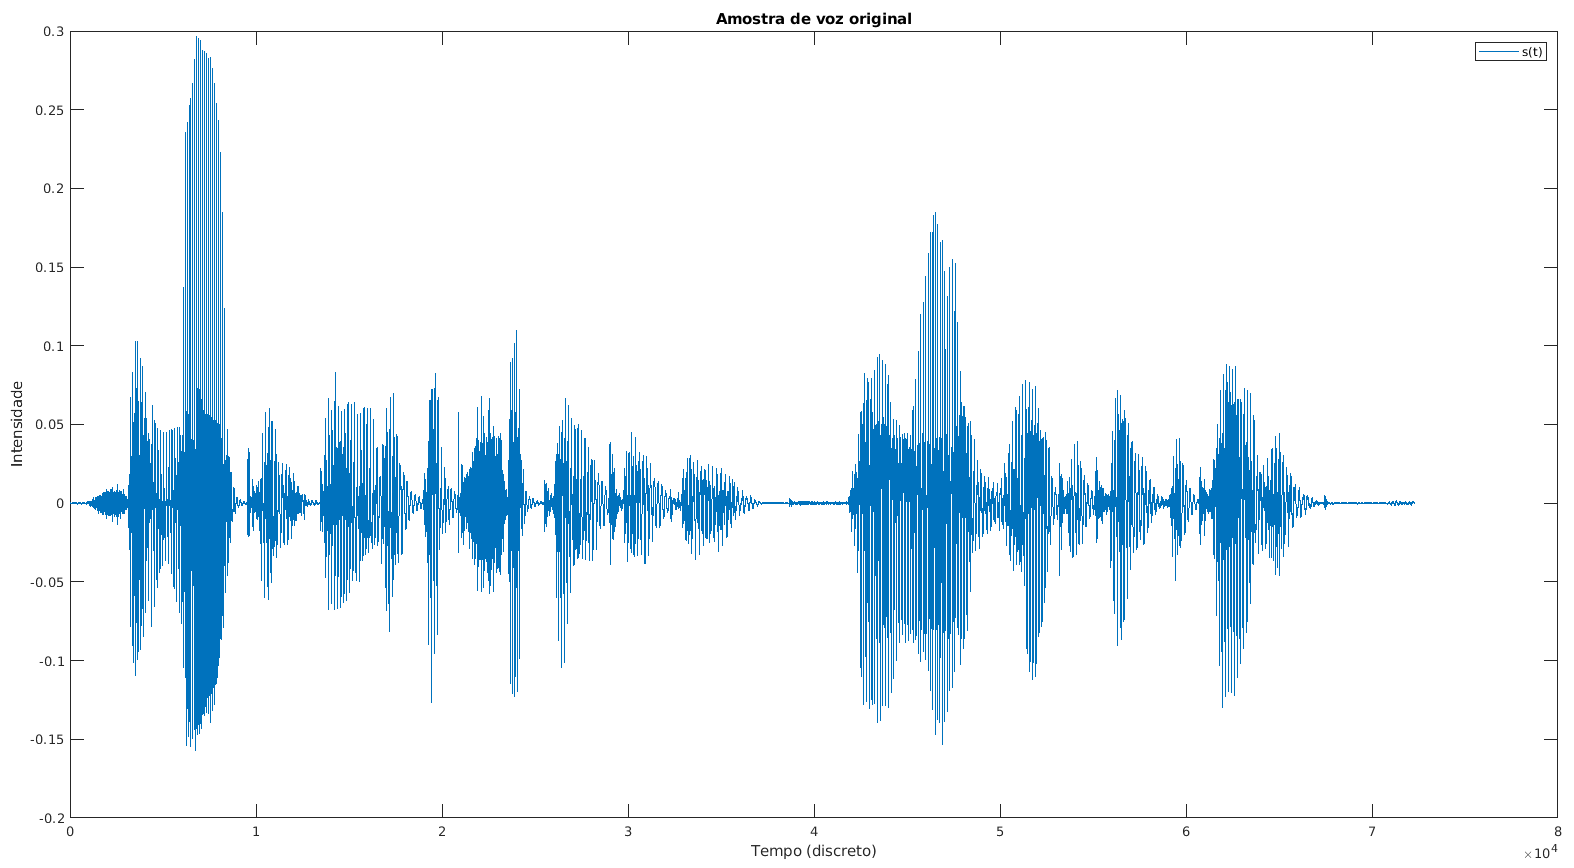
\includegraphics[scale=0.105]{voice-og-t2.png}
            \end{subfigure}
        \end{figure}

        \column{0.5\textwidth}
        \begin{figure}
            \begin{subfigure}{\textwidth}
                \centering
                \textattachfile{audios/voice-aug-riro-t2.wav}{\footnotesize amostra de voz reverberada - RIRO}
                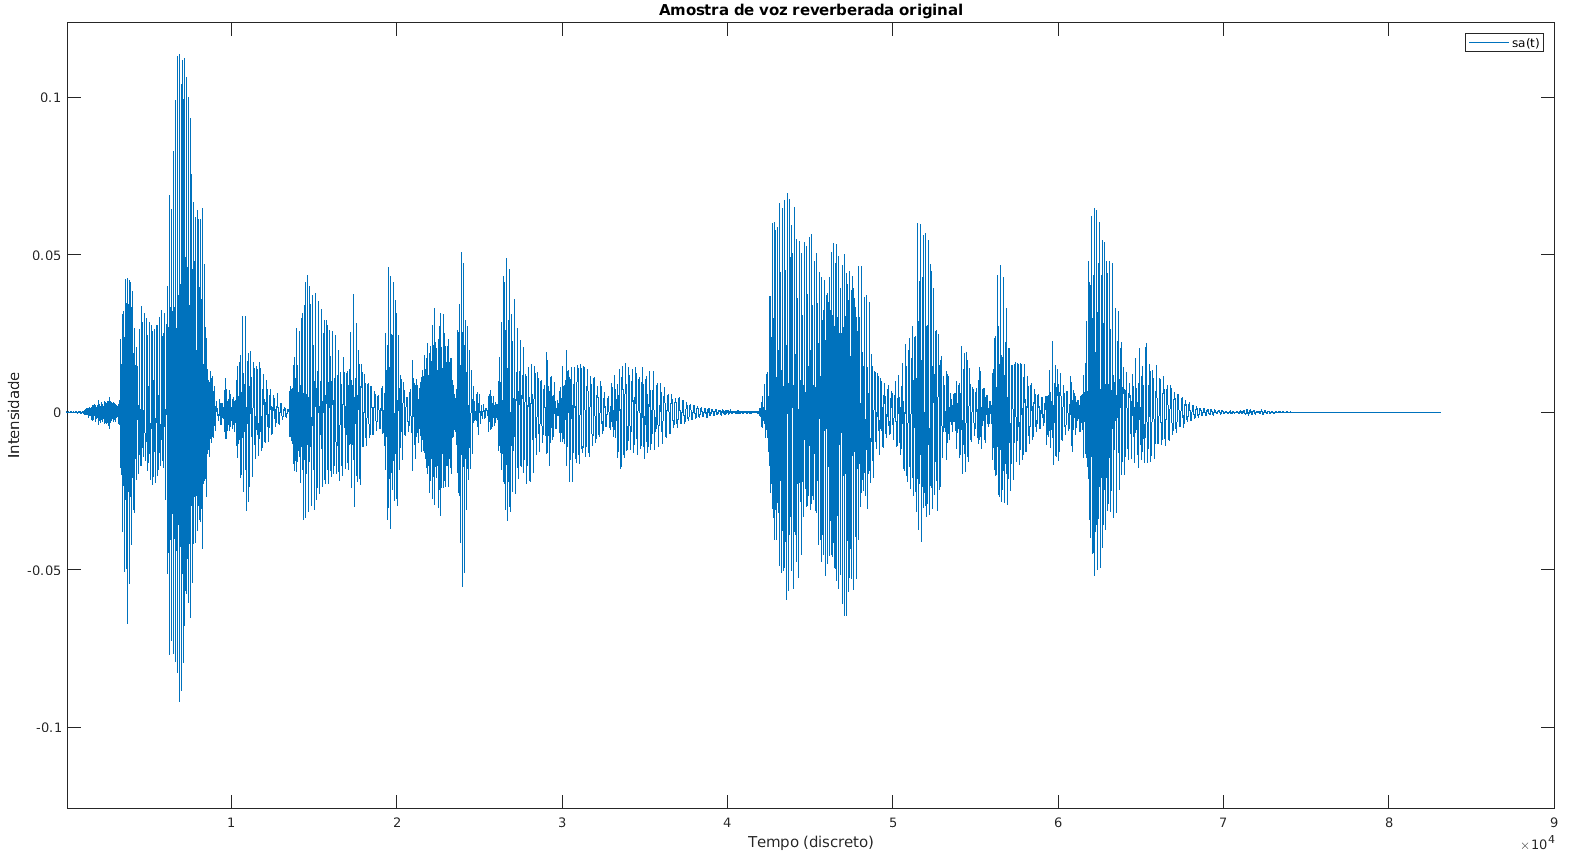
\includegraphics[scale=0.105]{voice-aug-riro-t2.png}
            \end{subfigure}
            \begin{subfigure}{\textwidth}
                \centering
                \textattachfile{audios/voice-aug-t2.wav}{\footnotesize amostra de voz reverberada - RIRSM}
                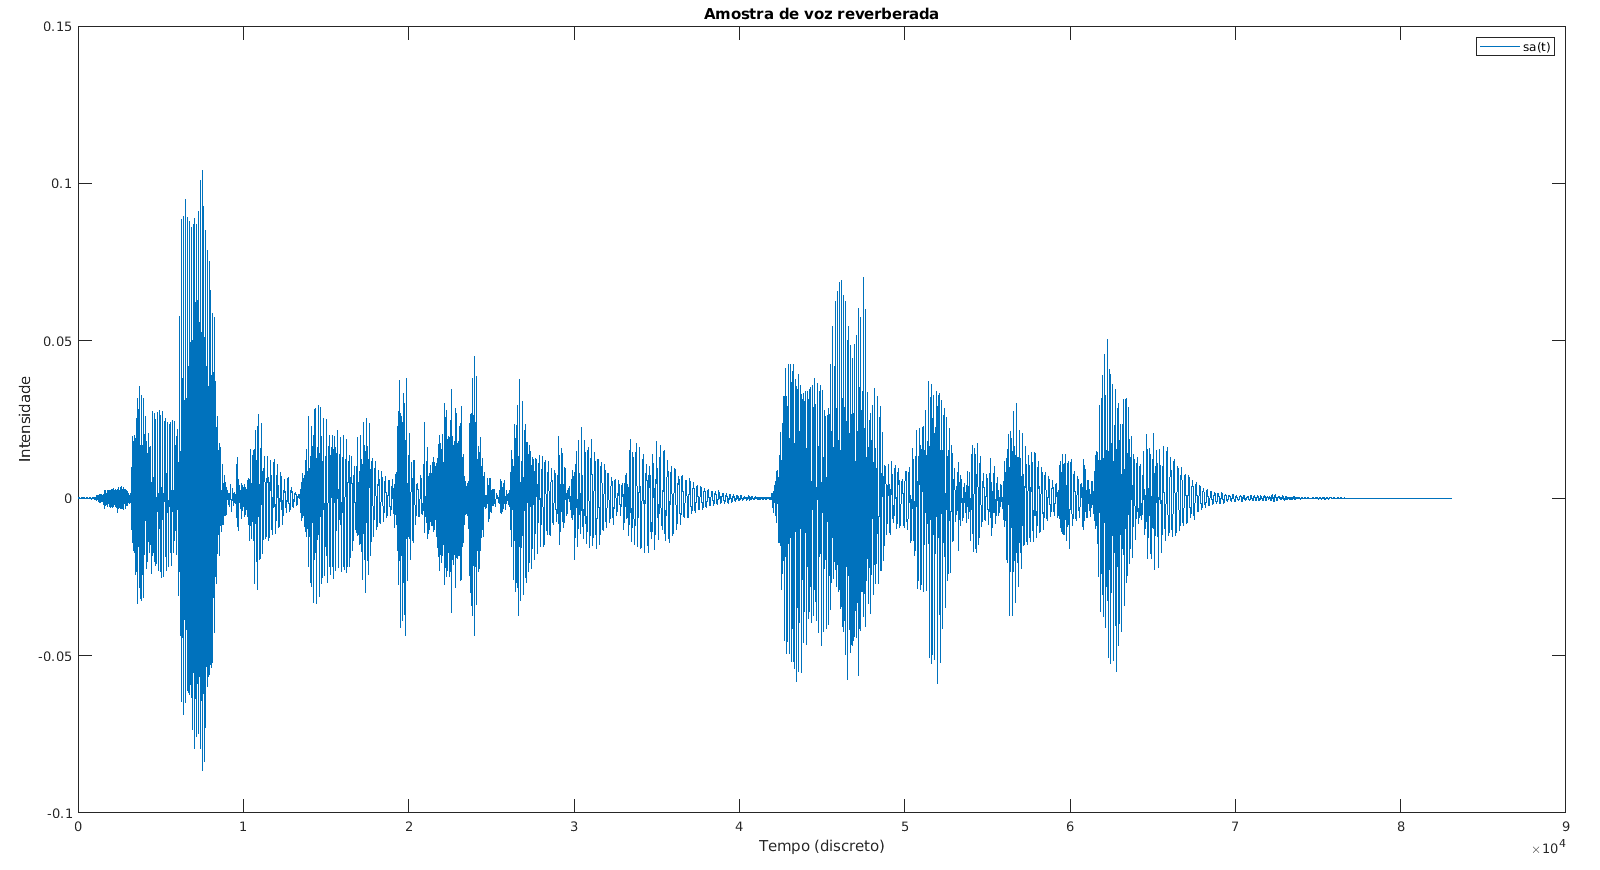
\includegraphics[scale=0.105]{voice-aug-t2.png}
            \end{subfigure}
        \end{figure}
    \end{columns}
\end{frame}

%% ---------------------------------------------------------------------------
% RESULTADOS - AVCD

\begin{frame}{Resultados - AVCD}
    \begin{table} [H]
        \centering
        \begin{tabular}{c|c|c|c|c|c}
    
            \textbf{Exemplo} & 
            \textbf{Sala RIR} & 
            \textbf{Distância (m)} &
            \textbf{AVA} &
            \textbf{SRP} &
            \textbf{SRF} \\
            \hline 
    
            N1 & lecture & 7.1 & M2-T1 & RP-6 & RF-1 \\
            N2 & booth & 1 & H2-T1 & RP-12 & RF-4 \\
            N3 & office & 2 & H1-T1 & RP-4 & RF-4 \\
            N4 & meeting & 1.7 & M1-T2 & RP-11 & RF-2 \\
            N5 & stairway & 1 & H2-T1 & RP-7 & RF-4 \\
    
        \end{tabular}
        \bigbreak
        \bigbreak
        \begin{tabular}{c|c|c|c|c|c}
    
            \textbf{Ex.} & 
            \textbf{$DRR_{org}$ (dB)} & 
            \textbf{$DRR_{res}$ (dB)} & 
            \textbf{$T60_{org}$ (s)} & 
            \textbf{$T60_{res}$ (s)} &
            \textbf{$SNR_{alvo}$} \\
            \hline 
    
            N1 & -4,5 & 17 & 1,38 & 0,56 & 5 \\
            N2 & 4,7 & 17 & 1,01 & 1,39 & 10 \\
            N3 & 0,5 & 14 & 0,75 & 0,60 & 14 \\
            N4 & 6,0 & 16 & 0,81 & 1,16 & 19 \\
            N5 & 5,0 & 18 & 2,70 & 3,68 & 3 \\
    
        \end{tabular}
    \end{table}
\end{frame}

\begin{frame}{Resultados - AVCD}
    \textbf{Experimento empírico}: análise subjetiva de nível de ruído, ordenado de mais para menos ruidoso.
    \vspace{1cm}
    
    \begin{table} [H]
        \centering
        \begin{tabular}{c|c|c}
    
            \textbf{Exemplo} & 
            \textbf{$SNR_{alvo}$ (s)} & 
            \textbf{Ordem} \\
            \hline 
    
            N1 &  5 & 3 \\
            N2 & 10 & 4 \\
            N3 & 14 & 1 \\
            N4 & 19 & 5 \\
            N5 &  3 & 2 \\
    
        \end{tabular}
    \end{table}
\end{frame}

\begin{frame}{Exemplo N4}
    \begin{columns}
        \column{0.5\textwidth}
        \begin{figure}
            \begin{subfigure}{\textwidth}
                \centering
                \textattachfile{audios/voice-og-n4.wav}{\scriptsize amostra de voz original}
                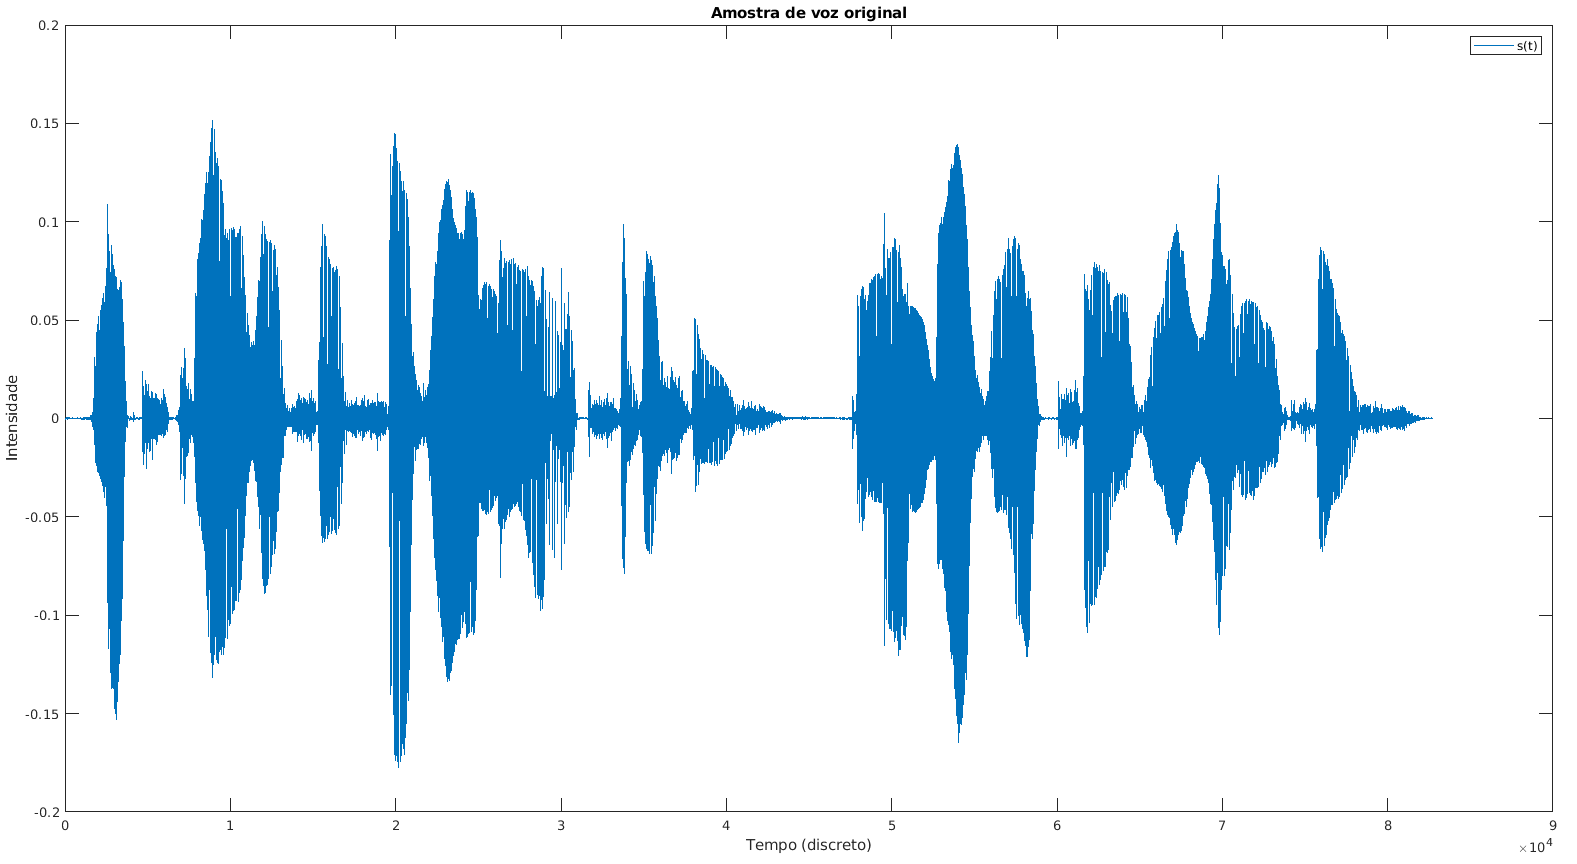
\includegraphics[scale=0.105]{voice-og-n4.png}
            \end{subfigure}
        \end{figure}

        \column{0.5\textwidth}
        \begin{figure}
            \begin{subfigure}{\textwidth}
                \centering
                \textattachfile{audios/voice-aug-n4.wav}{\footnotesize amostra de voz reverberada}
                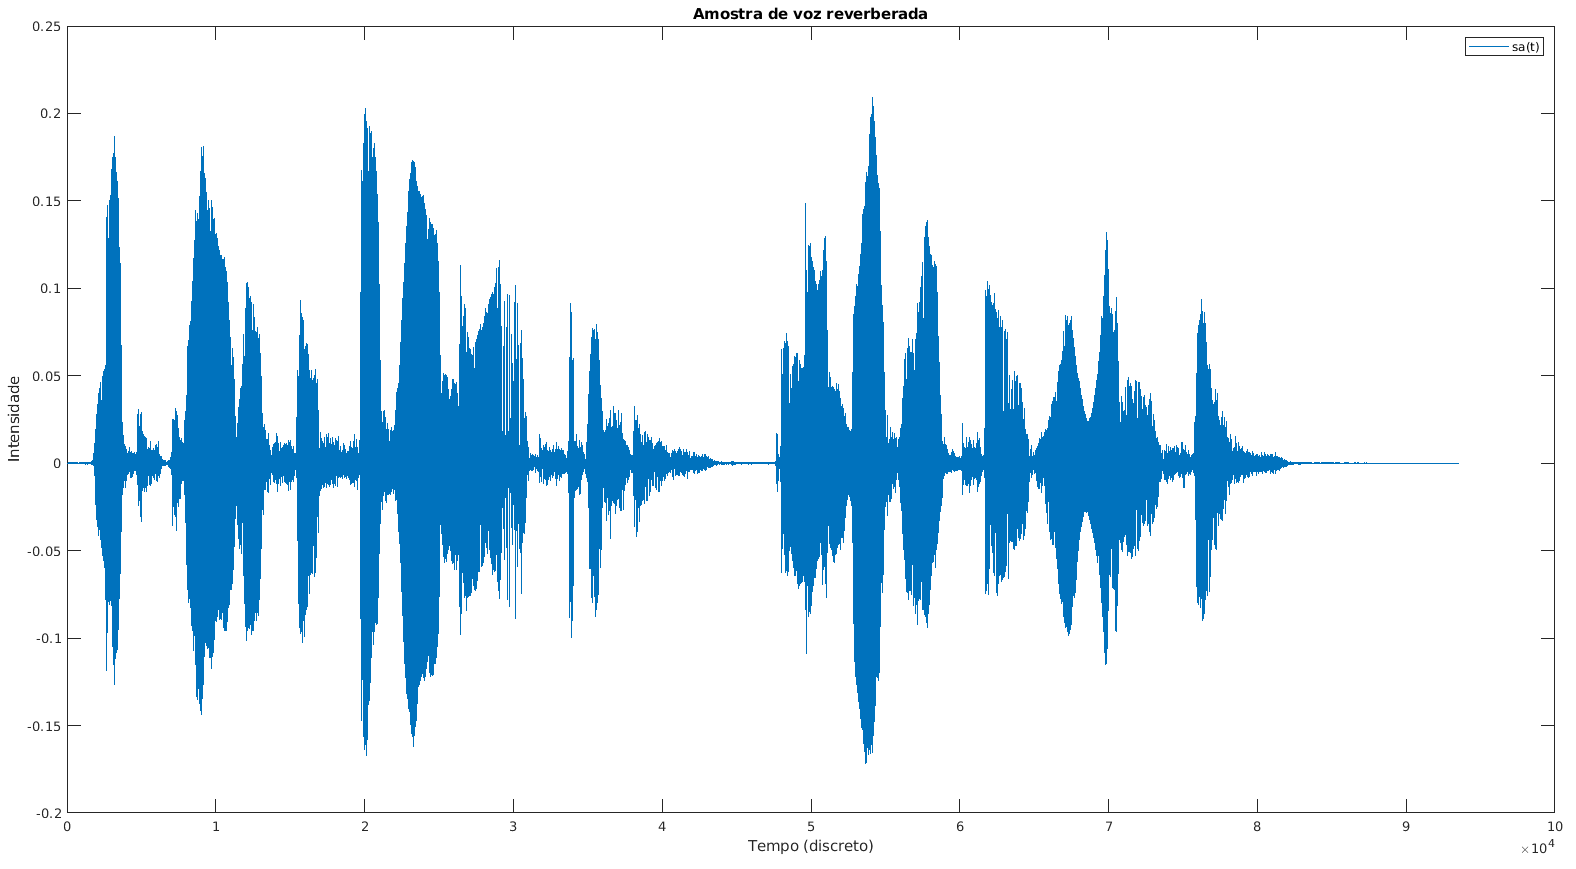
\includegraphics[scale=0.105]{voice-aug-n4.png}
            \end{subfigure}
            \begin{subfigure}{\textwidth}
                \centering
                \textattachfile{audios/voice-ns-n4.wav}{\footnotesize amostra de voz em campo distante}
                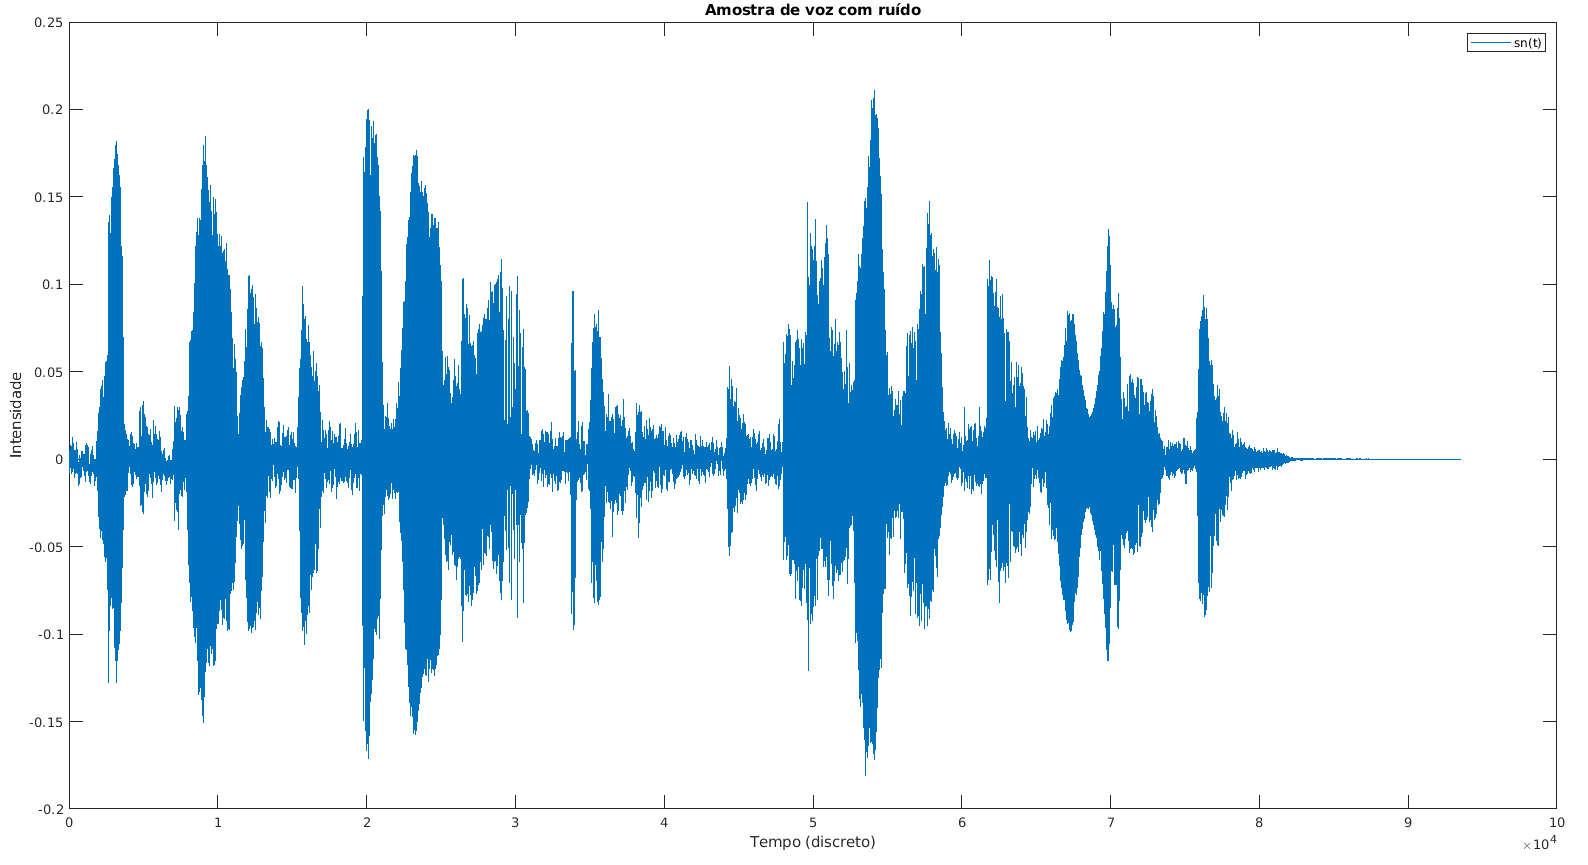
\includegraphics[scale=0.105]{voice-ns-n4.png}
            \end{subfigure}
        \end{figure}
    \end{columns}
\end{frame}

\begin{frame}{Exemplo N5}
    \begin{columns}
        \column{0.5\textwidth}
        \begin{figure}
            \begin{subfigure}{\textwidth}
                \centering
                \textattachfile{audios/voice-og-n5.wav}{\scriptsize amostra de voz original}
                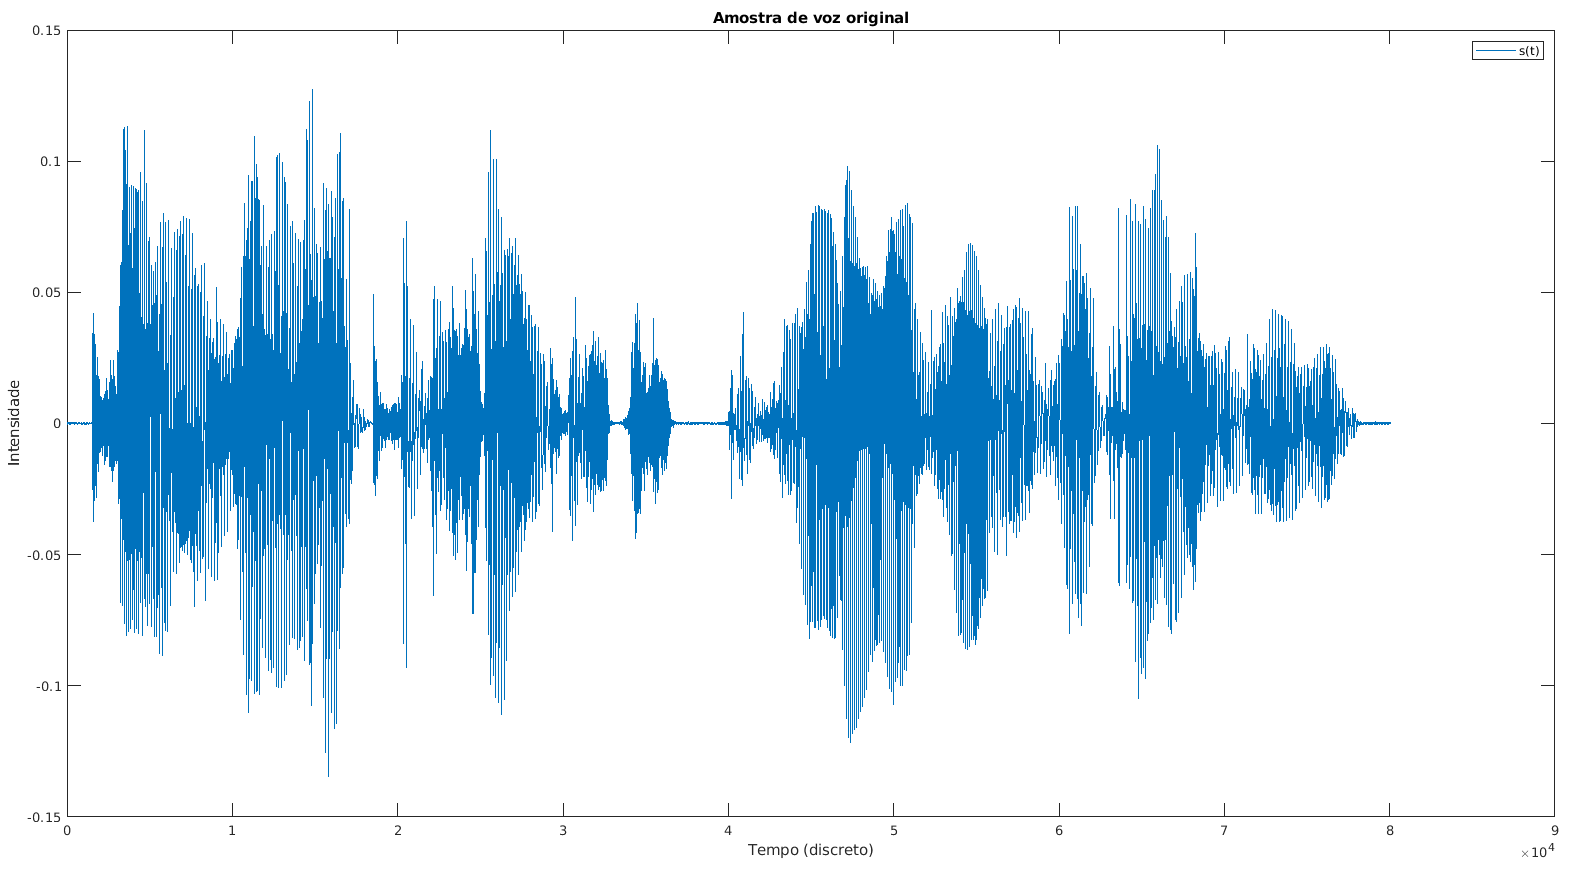
\includegraphics[scale=0.105]{voice-og-n5.png}
            \end{subfigure}
        \end{figure}

        \column{0.5\textwidth}
        \begin{figure}
            \begin{subfigure}{\textwidth}
                \centering
                \textattachfile{audios/voice-aug-n5.wav}{\footnotesize amostra de voz reverberada}
                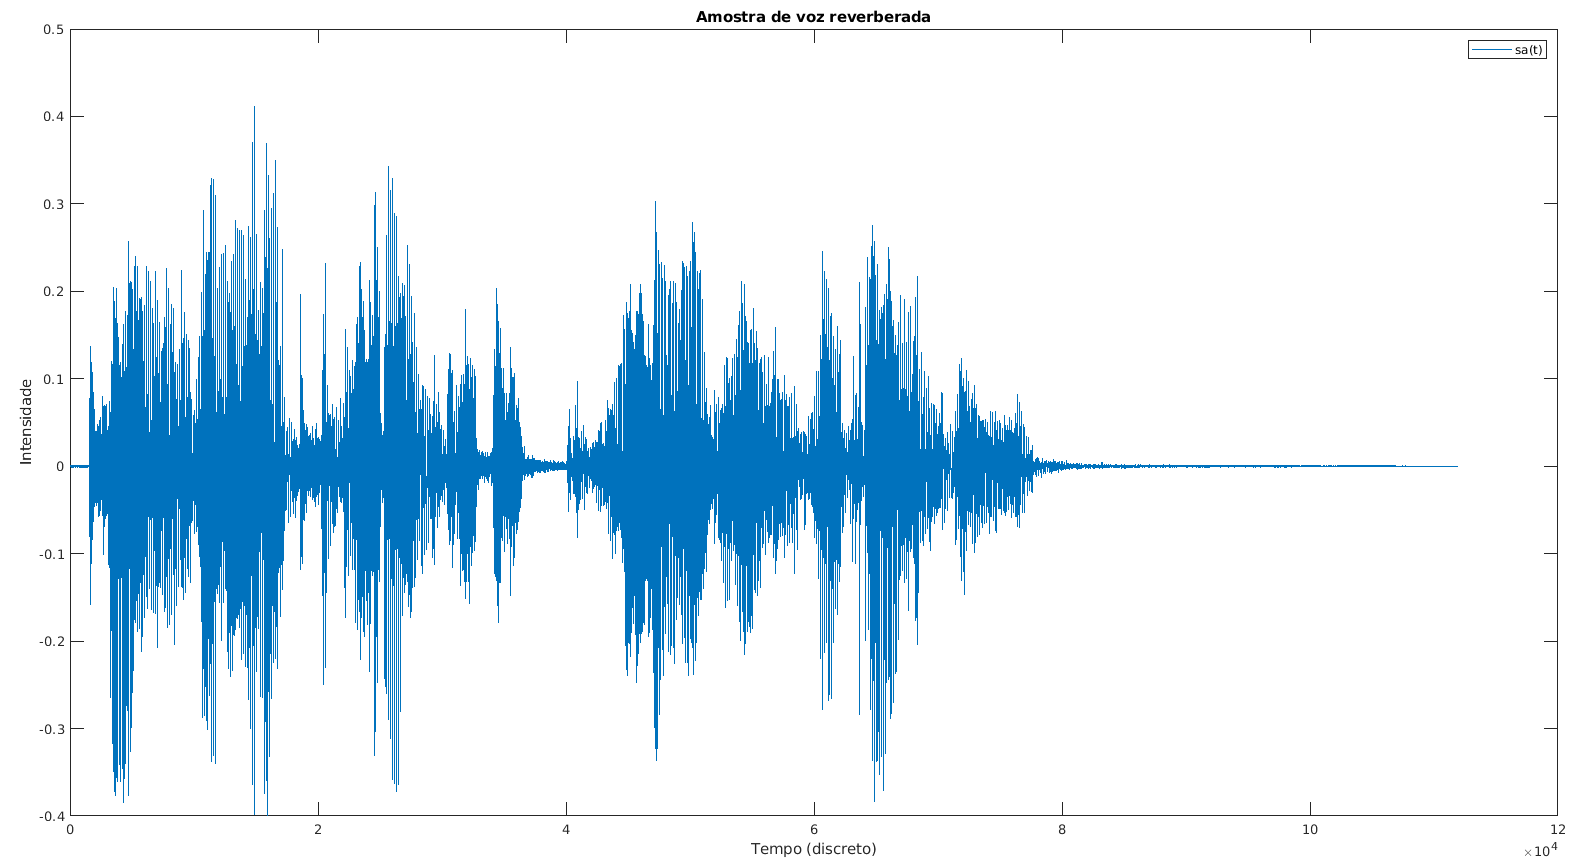
\includegraphics[scale=0.105]{voice-aug-n5.png}
            \end{subfigure}
            \begin{subfigure}{\textwidth}
                \centering
                \textattachfile{audios/voice-ns-n5.wav}{\footnotesize amostra de voz em campo distante}
                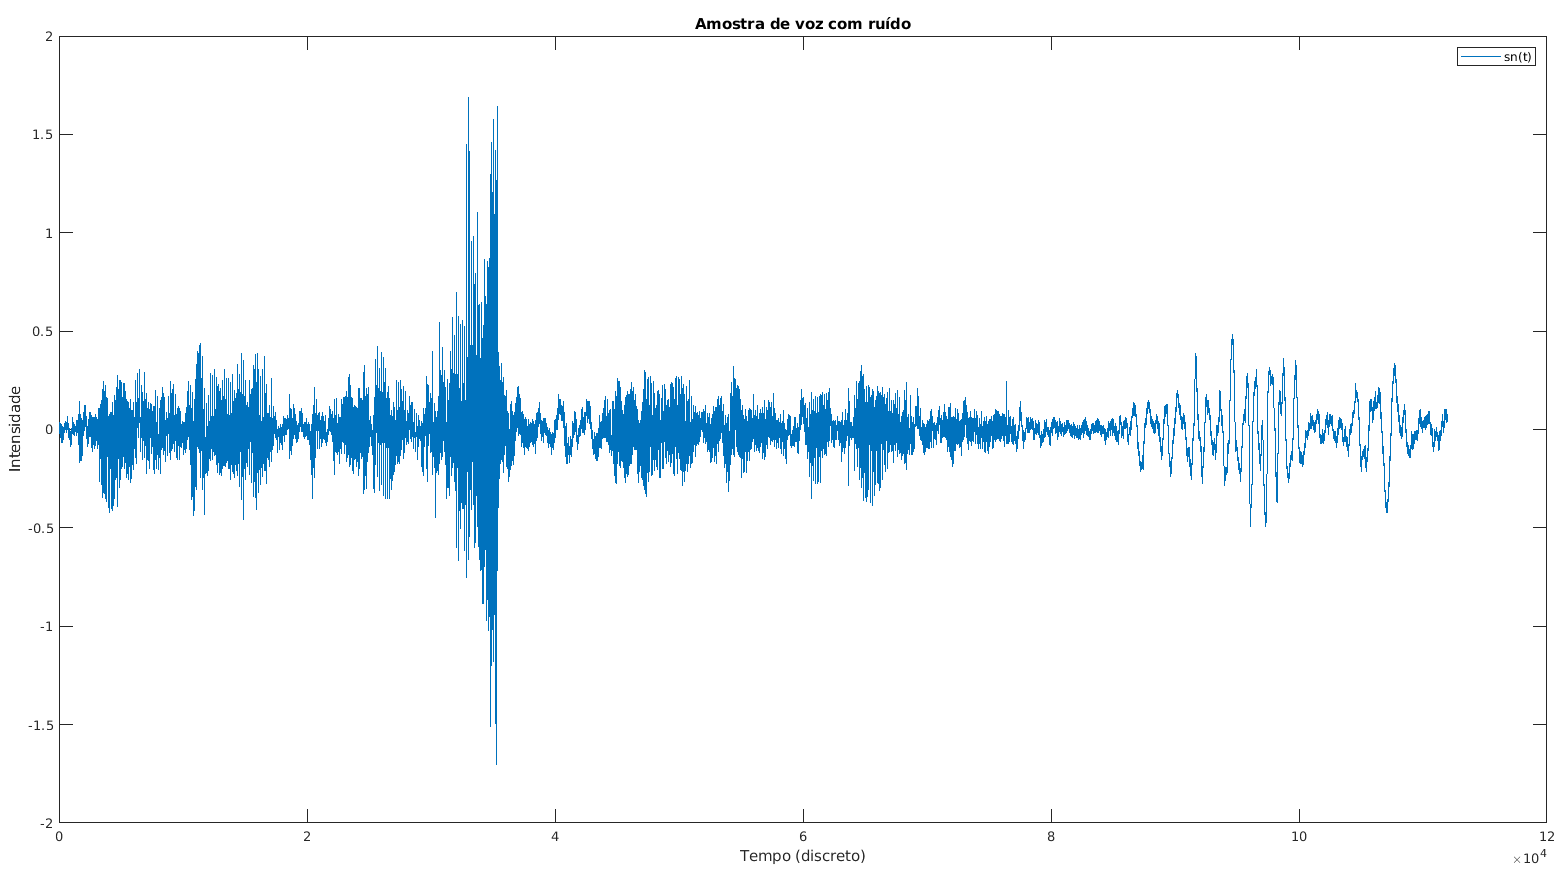
\includegraphics[scale=0.105]{voice-ns-n5.png}
            \end{subfigure}
        \end{figure}
    \end{columns}
\end{frame}

%% ---------------------------------------------------------------------------
% SECTION: Conclusão
\section{Conclusão}

\begin{frame} {Conclusões}
    \begin{itemize}
        \justifying
        \item Em grande parte, os resultados alcançados estão condizentes com os valores esperados.
        \item Discrepância nos valores de T60 podem ser explicados pelas diferenças de implementação entre este projeto e \cite{RIR_Data_Aug}.
        \item Avaliação empírica das sensações subjetivas de “distância” e “eco” condizentes com as modificações esperadas.
    \end{itemize}
\end{frame}

\begin{frame} {Trabalhos Futuros}
    \begin{itemize}
        \justifying
        \item Implementação de uma metodologia de \textit{data augmentation} de T60 mais próxima à usada no artigo \cite{RIR_Data_Aug}.
        \item Comparação entre as RIRs geradas com a metodologia implementada e RIRs geradas através de programas de simulação acústicas (RAIOS \cite{RAIOS}).
        \item Proposta de um modelo de rede de \textit{deep learning} para estimação de T60 e DRR em AVCDs para observação da eficácia das RIRs 
        como aprimoradoras do treinamento de redes neurais.
    \end{itemize}
\end{frame}

\begin{frame}
    \centering
    \huge{\textbf{\example{Obrigado!}}}
\end{frame}

%% ---------------------------------------------------------------------------
% Referências
\begin{frame}[allowframebreaks]
    \frametitle{Referências}
    \printbibliography
\end{frame}

\end{document}